\documentclass[a4paper,UKenglish]{lipics-v2018}
\nolinenumbers
%This is a template for producing LIPIcs articles. 
%See lipics-manual.pdf for further information.
%for A4 paper format use option "a4paper", for US-letter use option "letterpaper"
%for british hyphenation rules use option "UKenglish", for american hyphenation rules use option "USenglish"
% for section-numbered lemmas etc., use "numberwithinsect"
 
\usepackage{microtype}%if unwanted, comment out or use option "draft"

%\graphicspath{{./graphics/}}%helpful if your graphic files are in another directory

\bibliographystyle{plainurl}% the recommended bibstyle

%%%%%%%%%%%%%%%% OUR PRELIM STUFF BEGINS %%%%%%%%%%%%%%%%%%%%

\usepackage{courier}            % standard fixed width font
\usepackage[scaled]{helvet} % see www.ctan.org/get/macros/latex/required/psnfss/psnfss2e.pdf
% \usepackage{listings}          % format code
\usepackage{enumitem}      % adjust spacing in enums
\usepackage{xspace}
\usepackage{mathtools}
\usepackage{mathpartir}
\usepackage{amssymb}
\usepackage{amsmath}
\usepackage{latexsym}
\usepackage{graphicx}
% \usepackage[usenames,dvipsnames]{color}
\usepackage{listings}
\usepackage{subcaption}
\usepackage{stmaryrd}
\usepackage{comment}
\usepackage{float}
\usepackage{verbatimbox}
\usepackage{breakurl}
% \usepackage[breaklinks,draft=false,backref]{hyperref}
\hypersetup{
     colorlinks   = true,
     citecolor    = blue,
     linkcolor    = blue,
     urlcolor    = blue
}
\usepackage[multiple]{footmisc}

%--------------------------------------------------------------------
%Formatting Commands
%--------------------------------------------------------------------
\newcommand{\C}[1]{\code{#1}}
\renewcommand{\k}[1]{\mathtt{#1}} % Code font in math mode.
\newcommand{\code}[1]{\,{\tt #1}\,}
\newcommand{\conj}{\wedge}
\newcommand{\disj}{\vee}
\newcommand{\tuplee}[1]{\langle #1 \rangle}
\newcommand{\ALT}{~\mid~}
\newcommand{\lamb}[2]{\lambda #1.\,#2}
\newcommand{\spc}[0]{\quad}
\newcommand{\redsto}[3]{#1 \vdash #2 \longrightarrow #3}
\newcommand{\rredsto}[0]{\rightsquigarrow_r }
\newcommand{\evalsto}[0]{\longrightarrow }
\newcommand{\env}[0]{\Gamma}
\newcommand{\tywf}[2]{#1\,\vdash\,#2 \; \texttt{ok}}
\newcommand{\fgjtywf}[2]{#1\,\Vdash\,#2 \; \texttt{ok}}
\newcommand{\isvalid}[2]{#1\,\vdash\,#2}
\newcommand{\hastyp}[3]{#1\,\vdash\,#2:#3}
\newcommand{\hasfgjtyp}[3]{#1\,\Vdash^{}\,#2\,:\,#3}
\newcommand{\subtyp}[3]{#1\,\vdash\,#2 <: #3}
\newcommand{\fgjsubtyp}[3]{#1\,\Vdash\,#2 <: #3}
\newcommand{\msentails}[2]{#1\,\models\,#2}
\newcommand{\thesemof}[1]{ \llbracket #1 \rrbracket}
\newcommand{\subst}[2]{\lbrack #1/#2 \rbrack}
\newcommand{\absof}[1]{\thesemof{#1}}
\newcommand{\broom}{{\sc Broom}\xspace}
\newcommand{\name}{{\sc Broom}\xspace}
\newcommand{\namec}{{\sc Broomc}\xspace}
\newcommand{\fbname}{{\sc Featherweight Broom}\xspace}
\newcommand{\FB}{{\sc FB}\xspace}
\newcommand{\csharp}{C\#~}
\newcommand{\outlives}{\succeq}
\newcommand{\underlives}{\preceq}
\newcommand{\coloneqq}{::=}
\newcommand{\M}[1]{\mathtt{#1}}
\newcommand{\ObjZ}{\C{Object}}
\newcommand{\RgnZ}{\C{Region}}
\newcommand{\thisZ}{\C{this}}
\newcommand{\superZ}{\C{super}}
\newcommand{\unitZ}{\C{unit}}
\newcommand{\FuncZ}{\C{Func}}
\newcommand{\unitval}{\C{()}}
\newcommand{\inang}[1]{\langle #1 \rangle}
\newcommand{\rhoalloc}{\rho^a}
\newcommand{\rhobar}{\bar{\rho}}
\newcommand{\rhoallocm}{\rho^a_m}
\newcommand{\rhobarm}{\bar{\rho_m}}
\newcommand{\ralloc}{\pi^a}
\newcommand{\rgn}{r}
\newcommand{\rbar}{\bar{\rgn}}
\newcommand{\tbar}{\bar{T}}
\newcommand{\taubar}{\bar{\tau}}
\newcommand{\xbar}{\bar{x}}
\newcommand{\vbar}{\bar{v}}
\newcommand{\ebar}{\bar{e}}
\newcommand{\extends}{\triangleleft}
\newcommand{\rextends}{\blacktriangleleft}
\renewcommand{\bar}[1]{\overline{#1}}
\newcommand{\angR}{\inang{\rhobar \,|\, \phi}}
\newcommand{\angT}{\inang{\tbar}}
\newcommand{\tyvar}{a}
\newcommand{\tyvarb}{b}
\newcommand{\angAlpha}{\inang{\bar{\tyvar} \extends \bar{\fgjN}}}
\newcommand{\fgjN}{K}
\newcommand{\fbN}{N}
\newcommand{\headerOf}[1]{\C{class}\; #1\angAlpha\angR \extends \fbN}
\newcommand{\substFn}{\mathcal{S}}
% \newcommand{\regionSubstFn}{\mathcal{R}}
% \newcommand{\predSubstFn}{\mathcal{P}}
% \newcommand{\regionSubstFn}{\soln_V}
% \newcommand{\predSubstFn}{\soln_P}
\newcommand{\regionConstants}{R}
\newcommand{\regionVars}{V}
\newcommand{\predVars}{P}
\newcommand{\constraintSet}{C}
\newcommand{\regionDeltaMap}{{\Delta_R}}
\newcommand{\predDeltaMap}{{\Delta_P}}
\newcommand{\mang}{\inang{\bar{\rho_m} \,|\, \phi_m}}
\newcommand{\rhoset}{\Sigma}
\newcommand{\rhomap}{\Sigma}
\newcommand{\rhoenv}{\Delta}
\newcommand{\aenv}{\Theta}
\newcommand{\phicx}{\Phi}
\newcommand{\phictxt}{\phi_{cx}}
\newcommand{\phicstr}{\phi_{cs}}
\newcommand{\phisol}{\phi_{sol}}
\newcommand{\subtypcx}{\rhoenv,\aenv,\phicx}
\newcommand{\A}{{\mathcal{A}}}
\newcommand{\exptycx}[2]{\A,#1,#2}
\newcommand{\void}{\C{void}}
\newcommand{\functy}[3]{\FuncZ\inang{#1}\inang{#2,#3}}
\newcommand{\stmtsemcx}{\A,\env}
\newcommand{\stmtsemcxp}{\A',\env'}
\newcommand{\stmtsemcxpp}{\A'',\env''}
\newcommand{\sredsto}{\Rightarrow}
\newcommand{\stmtsem}[4]{#1 \, \vdash \, #2 \,/\, #3 \sredsto #4}
\newcommand{\okin}[2]{#1 \; \texttt{ok} \; \texttt{in} \; #2}
\newcommand{\lambdaexp}[4]{\lambda@#1\inang{#2}(#3). #4}
\newcommand{\Lambdaexp}[2]{\Lambda\inang{#1}.#2}
\newcommand{\letexp}[3]{\C{let}\;#1\,=\,#2\;\C{in}\;#3}
\newcommand{\letregion}[2]{\C{letregion}\;#1\;\C{in}\;#2}
\newcommand{\open}[4]{\C{open}\;#1\;\C{as}\; #3@#2\;\C{in}\;#4}
\newcommand{\opened}[3]{\C{opened}\;#1(#2)\;\C{in}\;#3}
\newcommand{\letd}[2]{\C{letd}\;#1\;\C{in}\;#2}
\newcommand{\unpackexp}[4]{\C{let}\;(#1,\,#2)\,=\,\C{unpack}\;#3\;\C{in}\;#4}
\newcommand{\invalidexn}{\bot}
\newcommand{\toprgn}{\pi_{\top}}
\newcommand{\csolvestar}{{\sc CSolve*}\xspace}
\newcommand{\elabExpr}{{\sf elabExpr}}
\newcommand{\fields}{{\sf fields}}
\newcommand{\mtype}{{\sf mtype}}
\newcommand{\mbody}{{\sf mbody}}
\newcommand{\bound}{{\sf bound}}
\newcommand{\fresh}{{\sf fresh}}
\newcommand{\typeOk}{{\sf typeOk}}
\newcommand{\subtypeOk}{{\sf subtypeOk}}
\newcommand{\templateTy}{{\sf templateTy}}
\newcommand{\allocRgn}{{\sf allocRgn}}
\newcommand{\shape}{{\sf shape}}
\newcommand{\ctype}{{\sf ctype}}
\newcommand{\override}{{\sf override}}
%\newcommand{\smallskip}{\vspace*{0.1in}}
\newcommand{\elabMeth}{{\sf elabMeth}}
\newcommand{\frv}{{\sf frv}}
\newcommand{\rv}{{\sf RVars}}
\newcommand{\solve}{{\sf solve}}
\newcommand{\valuee}{{\sf value}}
\newcommand{\elabClass}{{\sf elabClass}}
\newcommand{\elabCons}{{\sf elabCons}}
\newcommand{\elabClassTable}{{\sf elabClassTable}}
\newcommand{\CLOSED}{\mathtt{C}}
\newcommand{\OPEN}{\mathtt{O}}
\newcommand{\XFERRED}{{\color{blue}\times}}
\newcommand{\LIVE}{{\color{ForestGreen}\blacksquare}}
\newcommand{\SLIVE}{\LIVE}
\newcommand{\TLIVE}{\LIVE}
% \newcommand{\SLIVE}{{\color{ForestGreen}\widehat{\blacksquare}}}
% \newcommand{\TLIVE}{{\color{ForestGreen}\overrightarrow{\blacksquare}}}
%\newcommand{\FREE}{{\color{blue}\square}}
% \newcommand{\USED}{{\color{blue}\overrightarrow{\blacksquare}}}
\newcommand{\USED}{{\color{blue} \square}}
\newcommand{\transfer}{{\sf transfer}}
\newcommand{\CSP}{(C\lbrack \varphi,\rhobar \rbrack,\rhoenv_{\varphi}, \bar{\rhoenv})}
\newcommand{\csp}{(c\lbrack \varphi,\rhobar \rbrack,\rhoenv_{\varphi},\bar{\rhoenv})}
\newcommand{\Phicx}{\Phi_{cx}}
\newcommand{\Phics}{\Phi_{cs}}
\newcommand{\tynwf}[2]{#1\,\nvdash\,#2 \; \texttt{ok}}
\newcommand{\csid}[1]{\lbrack \mathbf{c_{#1}} \rbrack:\;}
\newcommand{\qqquad}{\quad\quad\quad}
\newcommand{\emptyA}[0]{(\Delta,\cdot,\phicx)}
\newcommand{\emptyASigp}[0]{(\Delta,\cdot,\phicx)}
\newcommand{\RgnZT}[1]{\RgnZ\inang{T}\inang{#1}}
\newcommand{\BZ}[0]{B\inang{\tbar}}
\newcommand{\BZT}[1]{B\inang{\tbar}\inang{#1}}
\newcommand{\redstoo}[3]{#2 \longrightarrow #3} %\Delta ignored
\newcommand{\redstocup}[3]{\redstoo{\rhoenv \cup \{#1\}}{#2}{#3}}
\newcommand{\loc}{\mathtt{l}}
\newcommand{\locbar}{\overline{\loc}}
\newcommand{\isLive}{{\sf isLive}}
\newcommand{\mem}{\Sigma}
\newcommand{\status}{s}
\newcommand{\toploc}{\loc_{\top}}
\newcommand{\consistent}{{\sf consistent}}

%Rules
%-----
\newcommand{\rulelabel}[1]{\textrm{\sc {#1}}}
\newcommand{\rulee}[1]{\textrm{\sc {#1}}}
\newcommand{\ilrulelabel}[1]{{\sc #1}}
\newcommand{\RULE}[2]{\frac{\begin{array}{c}#1\end{array}}
                           {\begin{array}{c}#2\end{array}}}

% Math mode
%-----------
\newenvironment{nop}{}{}
\newenvironment{smathpar}{
\begin{nop}\small\begin{mathpar}}{
\end{mathpar}\end{nop}\ignorespacesafterend}

\usepackage{listings}
\usepackage{subcaption}
\usepackage{stmaryrd}
\usepackage[skip=5pt]{caption}

\definecolor{Burgundy}{rgb}{0.5, 0.0, 0.13}
\definecolor{Bittersweet}{rgb}{1.0, 0.44, 0.37}
\definecolor{ForestGreen}{rgb}{0.13, 0.55, 0.13}
\definecolor{Bubbles}{rgb}{0.91, 1.0, 1.0}
\definecolor{LighterGray}{rgb}{0.93, 0.93, 0.93}

\newcommand{\lstjava}{\lstset{ %
language=Java, % choose the language of the code
backgroundcolor=\color{LighterGray},   
basicstyle=\footnotesize\ttfamily,       % the size of the fonts that are used for the code
keywordstyle=\color{Burgundy}\bf,
% numbers=left,                   % where to put the line-numbers
numberstyle=\tiny,      % the size of the fonts that are used for the line-numbers
stepnumber=1,                   % the step between two line-numbers. If it is 1 each line will be numbered
numbersep=5pt,                  % how far the line-numbers are from the code
showspaces=false,               % show spaces adding particular underscores
showstringspaces=false,         % underline spaces within strings
showtabs=false,                 % show tabs within strings adding particular underscores
% frame=single,                   % adds a frame around the code
tabsize=2,                      % sets default tabsize to 2 spaces
captionpos=b,                   % sets the caption-position to bottom
breaklines=true,                % sets automatic line breaking
breakatwhitespace=false,        % sets if automatic breaks should only happen at whitespace
commentstyle=\itshape\color{MidnightBlue},
%escapeinside={\%*}{*)},         % if you want to add a comment within your code
morekeywords={var, foreach, unit, letregion, let, in, as, openalloc, open, withroot, not, : , /\\}
}}
\lstnewenvironment{codejava}
    { % \centering
			\lstjava
      \lstset{mathescape=true}%
      \csname lst@setfirstlabel\endcsname}
    { %\centering
      \csname lst@savefirstlabel\endcsname}

\lstnewenvironment{numcodejava}
    { % \centering
			\lstjava
      \lstset{numbers=left,firstnumber=1}%
      \csname lst@setfirstlabel\endcsname}
    { %\centering
      \csname lst@savefirstlabel\endcsname}


%--------------------------------------------------------------------
%%%%%%%%%%%%%%%%%%%%%%%% OUR PRELIM STUFF ENDS %%%%%%%%%%%%%%%%%%%%%%
%--------------------------------------------------------------------

\title{Safe Transferable Regions}

\author{Gowtham Kaki}
       {Purdue University, USA\footnote{Work done during an internship at
Microsoft Research, India.}}
       {gkaki@purdue.edu}
       {}
       {}%mandatory, please use full name; only 1 author per \author macro; first two parameters are mandatory, other parameters can be empty.
\author{G. Ramalingam}
       {Microsoft Research, India}
       {grama@microsoft.com}
       {}
       {}%mandatory, please use full name; only 1 author per \author macro; first two parameters are mandatory, other parameters can be empty.

\authorrunning{G. Kaki and G. Ramalingam}%mandatory. First: Use abbreviated first/middle names. Second (only in severe cases): Use first author plus 'et al.'

\Copyright{Gowtham Kaki and G. Ramalingam}%mandatory, please use full first names. LIPIcs license is "CC-BY";  http://creativecommons.org/licenses/by/3.0/

\subjclass{
	\ccsdesc[500]{Software and its engineering~Allocation / deallocation strategies};\xspace
	\ccsdesc[500]{Software and its engineering~Object oriented languages};\xspace
	\ccsdesc[500]{Software and its engineering~Data flow languages};\xspace
	\ccsdesc[300]{Software and its engineering~Software verification and validation};\xspace
}% mandatory: Please choose ACM 1998 classifications from http://www.acm.org/about/class/ccs98-html . E.g., cite as "F.1.1 Models of Computation". 
\keywords{Memory Safety, Formal Methods, Type System, Type Inference,
Regions, Featherweight Java}% mandatory: Please provide 1-5 keywords

% Author macros::end %%%%%%%%%%%%%%%%%%%%%%%%%%%%%%%%%%%%%%%%%%%%%%%%%

\acknowledgements{We are grateful to Kapil Vaswani, Dimitrios
Vytiniotis, Michael Isard, and Steven Hand for their valuable inputs
during the initial stages of this project. We would also like to thank
multiple anonymous reviewers for their careful scrutiny and feedback
on various versions of this work.}%optional

%Editor-only macros:: begin (do not touch as author)%%%%%%%%%%%%%%%%%%%%%%%%%%%%%%%%%%
\EventEditors{Todd Millstein}
\EventNoEds{1}
\EventLongTitle{32nd European Conference on Object-Oriented Programming (ECOOP 2018)}
\EventShortTitle{ECOOP 2018}
\EventAcronym{ECOOP}
\EventYear{2018}
\EventDate{July 16--21, 2018}
\EventLocation{Amsterdam, Netherlands}
\EventLogo{}
\SeriesVolume{109}
\ArticleNo{11}
% Editor-only macros::end %%%%%%%%%%%%%%%%%%%%%%%%%%%%%%%%%%%%%%%%%%%%%%%

\begin{document}

\maketitle

%--------------------------------------------------------------------
%                           Abstract
%--------------------------------------------------------------------
\begin{abstract}
There is an increasing interest in alternative memory management
schemes that seek to combine the convenience of garbage collection and
the performance of manual memory management in a single language
framework.  Unfortunately, ensuring safety in presence of manual
memory management remains as great a challenge as ever. In this paper,
we present a C\#-like object-oriented language called {\sc
Broom}\xspace that uses a combination of region type system and
lightweight runtime checks to enforce safety in presence of
user-managed memory regions called \emph{transferable regions}. Unsafe
transferable regions have been previously used to contain the latency
due to unbounded GC pauses. Our approach shows that it is possible to
restore safety without compromising on the benefits of transferable
regions.  We prove the type safety of {\sc Broom}\xspace in a formal
framework that includes its C\#-inspired features, such as
higher-order functions and generics. We complement our type system
with a type inference algorithm, which eliminates the need for
programmers to write region annotations on types. The inference
algorithm has been proven sound and relatively complete. We describe a
prototype implementation of the inference algorithm, and our
experience of using it to enforce memory safety in dataflow programs.
\end{abstract}

%--------------------------------------------------------------------
%                           Introduction
%--------------------------------------------------------------------
\newcommand{\TODO}[1]{\textbf{TODO: #1}} \newcommand{\eg}{\emph{e.g.}}
\newcommand{\ie}{\emph{i.e.}}
\newcommand{\mypara}[1]{\textbf{#1}}

\section{Introduction} \label{sec:introduction}

% This paper presents a \emph{safe} and \emph{efficient} region-based approach
% to \emph{data transferable} between a set of concurrent actors, motivated by the following concerns.

Computations performed by a network of concurrent communicating actors
often involve data transfer between producers and consumers. Consider
for example the \C{SELECT} query operator shown in
Fig.~\ref{fig:motivating-eg}, which functions as an actor in a
dataflow computation involving a network of other such query
operators. \C{SELECT} receives a stream of input messages, each
associated with a time window $t$, processed by method
\texttt{onReceive}.  Each input message contains a list of inputs,
each processed by applying a user-defined function to create a
corresponding output.  Multiple messages with the same timestamp are
permitted and messages with different timestamps may arrive out of
order.  An invocation of method \texttt{OnNotify} indicates that no
more input messages with a timestamp $t$ will be subsequently
delivered.  At this point, the operator completes the processing for
time window $t$ and sends a corresponding output message to its
successor.

\mypara{Performance.}
When the transferred data structures are large, as is the case with many
streaming big-data analysis systems, garbage collection overhead becomes
significant~\cite{Broom:HotOS}.  Further, in a distributed
dataflow system, the GC pause at one node can have a cascading adverse
effect on the performance of other nodes~\cite{Broom:HotOS,harris15}:
a GC pause at an upstream actor can block downstream actors that are waiting for
messages.  However, much of the GC overhead results from the
collector performing avoidable or unproductive work.  For the example
in Fig.~\ref{fig:motivating-eg}, GC might repeatedly traverse the
\C{map}, although its objects cannot be collected until a
suitable timing message arrives.
There has been increasing interest in off-heap memory management for better performance
in the context of several  systems and languages (e.g.,
Spark~\cite{SPARK:2015}, Scala~\cite{ScalaOffHeap}, Rust).
Several systems (e.g.,~\cite{TRILL:2014}) resort to using ``free object pools'' to partially alleviate this problem, in
the absence of language support.

\begin{figure}[t!]
\begin{numcodejava}
class SelectVertex<TIn, TOut> {
  Func<TIn, TOut> selector;
  Dictionary<Time, List<TOut>> map;
  ...
  void onReceive(Time t, List<TIn> inList) {
    if (!map.ContainsKey(t)) map[t] = new List<TOut>();
    foreach (TIn input in inList) {
      TOut output = selector(input);
      map[t].add(output); } }
  void onNotify(Time t) {
     List<TOut> outList = map[t];
     map.Remove(t);
     transfer(successorId, t, outList); }
}
\end{numcodejava}
\caption{\C{SELECT} dataflow operator}
\label{fig:motivating-eg}
\vspace*{-0.2in}
\end{figure}

\begin{figure}
\centering
\subcaptionbox {
  Before transfer.
  \label{fig:after-transfer}
} [
  0.35\columnwidth
] {
  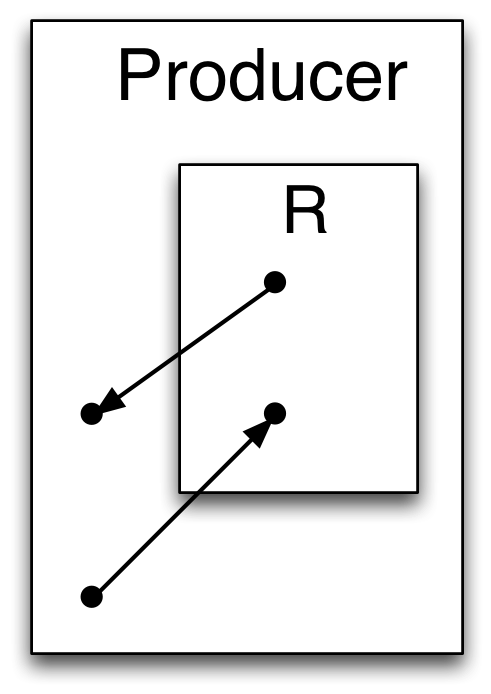
\includegraphics[scale=0.36]{producer-heap}
}
\subcaptionbox {
  After transfer.
  \label{fig:before-transfer}
} {
  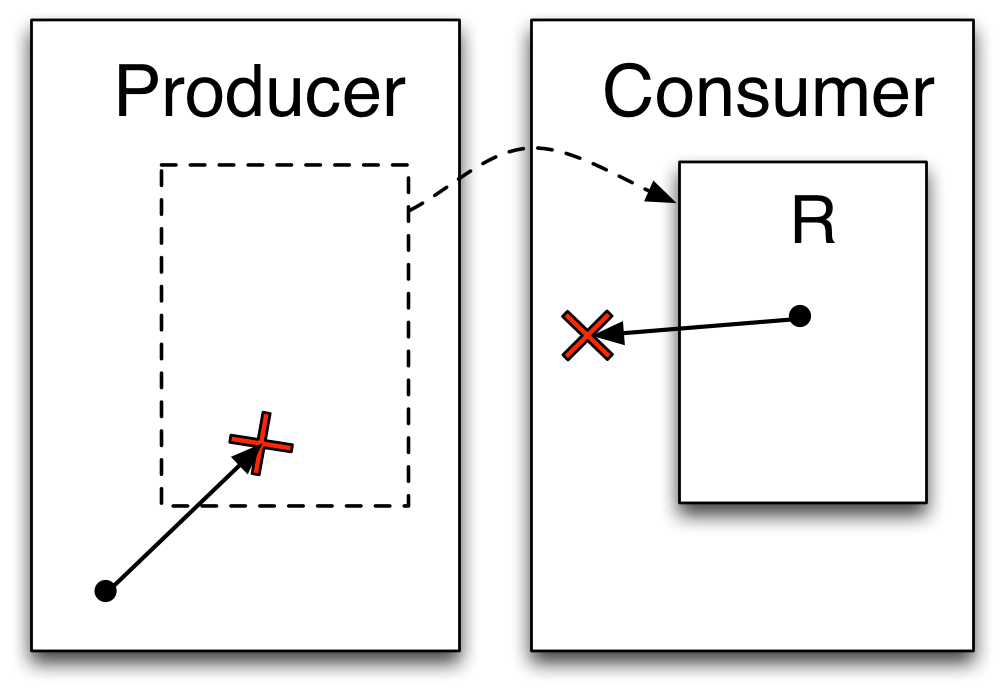
\includegraphics[scale=0.36]{producer-consumer-heap}
}

\caption{References in and out of a transferable region ($R$) become
invalid after transfer.}
\label{fig:transfer-violations}
\end{figure}

\mypara{Safety.}
Several of these systems are designed to allow the producer and
consumer to execute in the same address space or in different address
spaces (as determined by the compiler and runtime).  We wish to ensure
memory safety in the presence of such transferred data.  A transfer
operation, with no additional checks, may cause memory safety
violations, both at the producer of the data structure, and its
(possibly remote) consumer. At the producer, any existing references
into the transferred data structure become invalid post transfer. If
the data structure contains references to objects outside (the
transferred data), then such references become invalid in the context
of the consumer. Both scenarios are depicted in
Fig.~\ref{fig:transfer-violations}.  While references from within the
transferable data to outside can be disallowed in the interest of
safety, references into transferable data needs to be allowed before
the data is transferred. Allowing such references is crucial, as any
non-trivial program creates temporary references to the internal
objects of a data-structure.

\mypara{Safe Transferable Regions.}
In this paper, we present a language-based approach to cleanly
encapsulate transferable data and a safe and efficient implementation
of such data based on regions. 
%
A region is a block of memory that is allocated
and freed in one shot, often in constant time. A region may contain
one or more contiguous range of memory locations, and individual
objects may be dynamically allocated within the region over time,
while they are deallocated en masse when the region is freed.  Thus, a
region is a good fit for a transferable data-structure.  In
Fig.~\ref{fig:motivating-eg}, the output to be constructed for each
time window $t$ (i.e., \C{map[t]}) can be a separate region that is
allocated when the first message with timestamp $t$ arrives, and
deallocated after \C{map[t]} is transferred in \C{onNotify}.

The use of regions alleviates the performance concern related to
garbage collection described earlier. (It also enables more efficient
serialization/deserialization of data-structures across address spaces,
which is also a significant performance bottleneck in such systems.)
However, manual region memory management introduces memory safety
issues such as dangling pointers.
We present a single type system that simultaneously addresses
this safety concern, as well as those described above related to
the use of \emph{transferable data}.

Safe region-based memory management using types was
pioneered by Tofte and Talpin~\cite{tofte94,tofte97}, who 
use only lexically scoped regions.  At runtime, the set of all regions
(existing at a point in time) forms a stack. Thus, the lifetimes of
all regions must be well-nested: it is not possible to have two
regions whose lifetimes overlap, with neither one's lifetime contained
within the other.  Unfortunately, the data structures in the above
example do not satisfy this restriction (as the output messages for
multiple time windows may be simultaneously live, without any
containment relation between their lifetimes).  We refer to regions
with lexically scoped lifetimes as \emph{stack regions} and to regions
that do not have such a lexically scoped region as \emph{dynamic}
regions.

Our focus, in this paper, is on first-class \emph{memory-safe} dynamic regions
that can be safely transferred across address spaces. We refer to such dynamic
regions as \emph{transferable} regions.
%
Our approach is based on a variation of ideas introduced by~\cite{WW01,cyclone04}
that combine linear types and regions to support dynamic regions.
Unlike the prior work, we ensure memory safety in the presence of
transferable regions through a \emph{combination of a static
typing discipline and lightweight runtime checks in place of linear types}.

\mypara{Language.}
The cornerstone of this approach is an \C{open} lexical block for
transferable regions, that ``opens'' a transferable region and
guarantees that the region won't be transferred/freed while it is
open. By nesting a Tofte-Talpin style \C{letregion} lexical block,
that delimits the lifetime of a stack region, inside an \C{open}
lexical block for a transferable region, we can guarantee that the
transferable region will remain live as long as the stack region is
live. We say that the former \emph{outlives} the latter, and any
references from the stack region to the transferable region are
therefore safe. This is particularly useful, since such stack regions
serve as temporary working storage while working with the (opened)
transferable regions.

By controlling the outlives relationships between various
regions, we only allow safe cross-region references, while prohibiting
unsafe ones. In the above example, an outlives relationship
\emph{from} the stack region \emph{to} the transferable region means
that the references in that direction are allowed, but not the
references in the opposite direction. In contrast, if an \C{open}
block of a transferable region $R_0$ is nested inside an \C{open}
block of another transferable region $R_1$, we do not establish any
outlives relationships, thus declaring our intention to not allow any
cross-region references between $R_0$ and $R_1$.  Finally, we observe
that outlives relationships are established based on the lexical
structure of the program, hence a static type system can enforce them
effectively. By assigning region types to objects, which capture the
regions such objects are allocated in, and by maintaining outlives
relationships between various regions, we can statically decide the
safety of all references in the program.

\mypara{Type System.}
Formally, our type system introduces \emph{region parameters} (for both
classes and methods) and uses constrained parametric polymorphism
over these parameters, where the constraints capture outlives constraints
between the region parameters.
The type system may be seen as a form of ownership type system~\cite{OwnershipSurvey},
with a region being the owner of all objects allocated in that region.

\mypara{Lightweight Runtime Checks.}
Ensuring memory safety using this approach requires ensuring
that the use of transferable regions satisfies certain temporal properties.
Firstly, a transferable region should not be transferred/freed
inside an open block of that region (i.e, while it is still open).
Secondly, a transferred/freed region should not be opened. These are
typestate invariants on the transferable region objects, which are
hard to enforce statically in the presence of unrestricted
aliasing. Techniques like linear types and unique pointers can be used
to restrict aliasing, but the constraints they impose are often hard
to program around. We therefore enforce typestate invariants at
runtime via lightweight checks. In particular, we define an acceptable
state transition discipline for transferable regions
(Fig.~\ref{fig:region-fsm}), and check, at runtime, whether a given
transition of a transferable region (\eg, from \emph{open} state to
\emph{freed} state) is valid or not. The check is lightweight since it
only involves checking a single tag that captures the current state.
We believe that this is a reasonable choice since regions are
coarse-grained objects manipulated infrequently, when compared to the
fine-grained objects that are present inside these regions, for which
safety is enforced statically. 

\mypara{Type Inference.}
One of the key contributions of this paper is a type inference
algorithm that eliminates the need for users to write region type
annotations.  The users write programs in the underlying language that
provides primitives for the users to manipulate regions (create, open,
free, transfer) and to allocate objects in regions, but has no region
type annotations.

Our inference algorithm proceeds in three stages: in the first stage,
we elaborate the program by introducing region parameters (for classes
and methods); in the second stage we generate a set of constraints
that must be satisfied for the program to type check; in the third
stage, we solve the set of constraints, inferring the preconditions of
all classes and methods (in terms of the expected outlives-constraints
between the region parameters).  We show that the algorithm is sound,
and the stages of constraint generation and solving are complete
(i.e., the algorithm is complete relative to the first stage of
elaboration).
% (using an interprocedural fixed point computation).

\mypara{Evaluation.}
Our work was inspired by~\cite{Broom:HotOS}, which presents evidence
that realistic programs can be written using transferable regions and
that this can yield significant performance improvements.
While~\cite{Broom:HotOS} addresses the engineering challenges in
extending a managed runtime with transferable regions, it adopts an ad
hoc approach insofar as language design is concerned, exposing the
region functionality through an unsafe API, and in the process losing
the safety guarantees. Our contribution is an alternative approach
that is grounded in sound theory and restores the language safety
guarantees. The utility of our approach is demonstrated by a prototype
implementation of our type inference algorithm that was able to
identify unsafe memory accesses among the benchmarks extracted
from~\cite{Broom:HotOS}.  

\mypara{Contributions.}
The paper makes the following contributions:

\begin{itemize} 
  \item We present \broom, a \csharp-like typed object-oriented
  language that supports programmer-managed memory regions. \broom{}
  extends its core language, which includes \emph{lambdas}
  (higher-order functions) and \emph{generics} (parametric
  polymorphism), with constructs to create, manage and free static and
  transferable memory regions. Transferable regions are first-class
  values in \broom.

\item \broom{} is equipped with a region type system that statically
  guarantees safety of all memory accesses in a well-typed program,
  provided that certain typestate invariants on regions hold.  The
  latter invariants are enforced via simple runtime checks.

  \item We define an operational semantics for \broom, and a type
  safety result that clearly defines and proves safety guarantees
  described above.

  \item We describe a region type inference algorithm for \broom that
  (a). completely eliminates the need to annotate \broom programs with
  region types, and (b). enables seamless interoperability between
  region-aware \broom programs and legacy standard library code that
  is region-oblivious. Our inference algorithm is based on a novel
  constraint solver that performs abduction in a partial-order
  constraint domain to infer weakest solutions to recursive
  constraints.

\item We establish the soundness and relative completeness of the type
inference algorithm.

  \item We describe an implementation of \broom frontend in OCaml,
  along with case studies where the region type system was able to
  identify unsafe memory accesses statically.
  
\end{itemize}


%--------------------------------------------------------------------
%                             Overview
%--------------------------------------------------------------------
\newcommand{\COMMENT}[1]{}

\section{An Informal Overview of \name} \label{sec:overview}

\name enriches a simple object-oriented language (supporting
parametric polymorphism and lambdas) with a set of region-specific
constructs.  In this section, we present an informal overview of these
region-specific constructs.

\subsection{Using Regions in \name}
\label{sec:alloc-ctxt}

\mypara{Stack Regions} The ``\C{letregion R \{ S \}}'' construct
creates a new stack region, with a static identifier \C{R}, whose
scope is restricted to the statement \C{S}. The semantics of
\C{letregion} is similar to Tofte and Talpin~\cite{tofte94}'s
\C{letregion} expression: objects can be allocated by \C{S} in the
newly created region while \C{R} is in scope, but the region and all
objects allocated within it are freed at the end of \C{S}.

\mypara{Object Allocation} The ``\C{new@R T()}'' construct creates
a new object of type \C{T} in the region \C{R}. The specification of
the allocation region \C{R} in this construct is optional.  At
runtime, \name maintains a stack of \emph{active} regions, and we
refer to the region at the top of the stack as the \emph{allocation
context}. The statement \C{new T()} allocates the newly created object
in the current allocation context.
%
This is important as it enables \name applications to use existing
region-oblivious C\# libraries, as explained soon.

\mypara{Transferable Regions} 
Transferable regions are first class values of \name: they are objects
of the class \C{Region}, they are created using the \C{new} keyword,
and can be passed as arguments, stored in data structures, and
returned from methods.  A transferable region is intended to
encapsulate a single data-structure, consisting of a collection of
objects with a distinguished root object of some type \C{T}, which we
refer to as the region's \emph{root} object.  The class \C{Region} is
parametric over the type \C{T} of this root object.

The \C{Region} constructor takes as a parameter a function that
constructs the root object: it creates a new region and invokes this
function, with the new region as the allocation context, to create the
root object of the region. The following code illustrates the
creation of a transferable region, whose root is an object of type
\C{A}.
% (\C{r}) of type \C{T}:
\begin{codejava} 
  Region<A> rgn = new Region<A>(() => new A())
\end{codejava} 
In the above code, \C{rgn} is called the \emph{handler} to the newly
created region, and is required to read the contents of the region, or
change its state. The class \C{Region} offers two methods: a \C{free}
method that deallocates the region (and all the objects allocated
within it), and \C{transfer} method that transfers the region to a
(possibly remote) consumer process. 

\mypara{Open and Closed Regions} A transferable region must be
explicitly \emph{opened} using \name's \C{open} construct in order to
either read or update or allocate objects in the region.
Specifically, the construct ``\C{open rgn as v@R \{ S \}}'' does the
following: (a). It opens the transferable region handled by \C{rgn}
for allocation (i.e., makes it the current allocation context), (b).
binds the identifier \C{R} to this open region, and (c). initializes
the newly introduced local variable \C{v} to refer to the root object
of the region.  The \C{@R} part of the statement is optional and may
be omitted.  The \C{open} construct is intended to simplify the
problem of ensuring memory safety, as will be explained soon.  We
refer to a transferable region that has not been opened as a
\emph{closed} region. A transferable region can only be transferred or
freed when it is in closed state. The acceptable state transition
discipline over the lifetime of a transferable region is described
in Fig.~\ref{fig:region-fsm}. Enforcement of this discipline is done
at runtime.

Opening a region also makes it the current allocation context.
Thus, given a  C\# library function \C{f} (that makes no use of \name's region constructs),
opening a region \C{R} and invoking \C{f} has the effect that all objects created by this
invocation are allocated in the region \C{R}.

\mypara{Motivating Example}
Fig~\ref{fig:motivating-eg-in-broom} shows how the motivating example
of Fig.~\ref{fig:motivating-eg} can be written in \name. The
\C{onReceive} method receives its input message in a
\emph{transferred} region (\ie, a \emph{closed} region whose ownership
is transferred to the recipient). On Line 7, we create a new region to
store the output for time \C{t}, initializing it to contain an empty
list. On Lines 8 and 9, we open the input region \C{inRgn} followed by
creating a new stack region \C{R0}. The temporary objects created by
the iteration on line 10, for example, will be allocated in the stack
region \C{R0} that lives just long enough.  We open the desired output
region on line 11, so that the new output objects created by the
invocation of \C{selector} on line 12 are allocated in the output
region.  Finally, the input region is freed on line 14. The output
region at \C{map[t]} stays as along as input messages with timestamp
\C{t} keep arriving. When the timing message for \C{t} arrives, the
\C{onNotify} method transfers the \C{outRgn} at \C{map[t]} to a
downstream actor.

\begin{figure}[t!]
\begin{numcodejava}
class SelectVertex<TIn, TOut> {
  Func<TIn, TOut> selector;
  Dictionary<Time, Region<List<TOut>>> map;
  ...
  void onReceive(Time t,Region<List<TIn>> inRgn){
    if (!map.ContainsKey(t))
       map[t] = new Region<List<TOut>> (() => new List<TOut>());
    open inRgn as inList {
      letregion R0 {
        foreach (TIn input in inList) {
          open map[t] as outList {
            TOut output = selector(input);
            outList.add(output); } } } }
    inRgn.free();
  }
  void onNotify(Time t) {
     Region<List<TOut>> outRgn = map[t];
     map.Remove(t);
     outRgn.transfer(successorId);
  }
}
\end{numcodejava}
\caption{\C{SELECT} dataflow operator in \name}
\label{fig:motivating-eg-in-broom}
\vspace*{-0.15in}
\end{figure}

\begin{figure} 
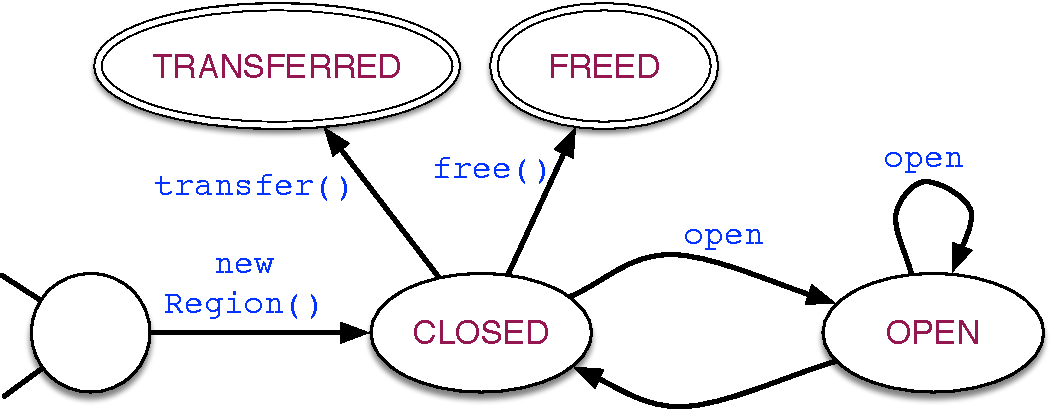
\includegraphics[scale=0.45]{region-fsm}
\caption{The lifetime of a dynamic (transferable) region in \name}
\label{fig:region-fsm} 
\vspace*{-0.1in} 
\end{figure}

\begin{figure*}[t!]
%
\begin{smathpar}
\renewcommand{\arraystretch}{1.2}
\begin{array}{lclcl} 
\multicolumn{5}{c}{
  {\pi} \in \mathtt{Region\; identifiers} \qquad
  {\rho} \in \mathtt{Region \; variables} \qquad
% {\loc} \in \mathtt{Memory\; locations}
  {\tyvar, \tyvarb} \in \mathtt{Type \; variables}}\\
\multicolumn{5}{c}{
% {\tyvar, \tyvarb} \in \mathtt{Type \; variables} \qquad
  {m} \in \mathtt{Method \; names} \qquad
  {x,y,f} \in \mathtt{Variables \; and \; fields} }\\
cn & \in & \M{Class \; names} & \coloneqq & \ObjZ \ALT \RgnZ \ALT A \ALT B\\
     \fgjN & \in & \M{FGJ \; class \; types} & \coloneqq & cn\inang{\tbar}\\
T  & \in & \M{FGJ \; types} & \coloneqq & \tyvar \ALT  \fgjN \ALT \unitZ
     \ALT \bar{T} \rightarrow T \\
r  & \in & \M{Region\; annotations} & \coloneqq & \rho \ALT \pi \\
% \status & \in & \mathtt{Region\; Typestate} & \coloneqq & \FREE \ALT
%                   \USED \ALT \LIVE \ALT \XFERRED\\
\fbN  & \in & \M{Annotated \; class \; types} & \coloneqq & 
     cn\inang{\tbar}\inang{\rbar} \\
\tau &\in& \M{types} & \coloneqq & T@\rgn  
      \ALT \fbN \ALT \unitZ 
      \ALT \inang{\rhobar \,|\, \phi}\bar{\tau}
      \xrightarrow{\rgn} \tau \\
C  & \in & \M{Class \; definitions} & \coloneqq & 
     \C{class} \; cn\inang{\bar{\tyvar} \extends \bar{\fgjN}} 
                    \inang{\rhobar \,|\, \phi}\extends \fbN 
                    \{\bar{\tau} \; \bar{f};\; \bar{d}\}\;\\
d  & \in & \M{Methods} & \coloneqq & 
     \tau \; m\inang{\rhobar \,|\, \phi} (\taubar \; \xbar)
     \{\C{return}\;e;\}\\
\phi,\phicx &\in& \M{Region\;constraints} & \coloneqq & true 
      \ALT \rgn \outlives \rgn \ALT \rgn = \rgn \ALT \phi \conj \phi\\
e  & \in & \M{Expressions} & \coloneqq &
     \unitval \ALT x \ALT e.f 
     \ALT e.m\inang{\rbar}(\ebar) \ALT \C{new}\;\fbN(\ebar)
 \\  & & & & 
     \ALT \lambdaexp{\rgn}{\rhobar \,|\, \phi}  {\xbar:\taubar} {e}
     \ALT e\inang{\rbar}(\bar{e})
     \ALT \letexp{x}{e}{e}
 \\  & & & & 
     \ALT \letregion{\pi}{e} 
      \ALT \open{e}{\pi}{y}{e}\\
%  & & & & \ALT \letd{\loc}{e} \ALT \opened{\loc}{\status}{e}\\
\end{array}
\end{smathpar}

\caption{\fbname: syntax}
\label{fig:fb-syntax}
\end{figure*}

\mypara{Cloning} Note that in the example from
Fig.~\ref{fig:motivating-eg-in-broom} the object returned by the
\C{selector} (on Line 12) should not contain any references to the
input object, since the input region, where the object resides, will
be freed at the end of the method. If there is a need for the output
object to point to subobjects of the input object, such subobjects
must be cloned (to copy them from the input region to the output
region).  Fortunately, \name's region type system
(\S~\ref{sec:type-system}) is capable of capturing such nuances in the
type of \C{selector} and the type checker will ensure correctness.
Furthermore, the type can be automatically inferred by \name's region
type inference (\S~\ref{sec:type-inference}), which can perform the
above reasoning on behalf of the programmer.

%--------------------------------------------------------------------
%                             Type System
%--------------------------------------------------------------------
\section{\fbname}
\label{sec:type-system}

The purpose of \name's region type system is to enforce the key
invariant required for memory safety, namely that an object $o_1$ in a
region $R_1$ contains a reference to an object $o_2$ in $R_2$, only if
$R_2$ is guaranteed to outlive $R_1$.  While the invariant is easily
stated, enforcing it in the presence of first-class dynamic regions,
parametric polymorphism (generics), and higher-order functions
requires new reasoning principles that we formally develop in this
section. We introduce \fbname (\FB), an explicitly typed core language
(with region types) that incorporates the features introduced in the
previous section. \fbname builds on the Featherweight Generic Java
(FGJ)~\cite{fgj} formalism, and reuses notations and various
definitions from~\cite{fgj}, such as the definition of type
well-formedness for the core (region-free) language.  (The language
used in Section~\ref{sec:overview} is essentially a version of FGJ
without region types and with some syntactic sugar.)

\subsection{Syntax}
\label{sec:fb-syntax}

Fig~\ref{fig:fb-syntax} describes the syntax of \FB.
We refer to the class types of FGJ as \emph{core types}.
%
The following definition of \C{Pair} class in \FB illustrates some of
the key elements of the formal language (the symbol $\extends$ should
be read \emph{extends}, and the symbol $\outlives$ stands for
\emph{outlives}):
\begin{codejava}[mathescape=true]
class Pair<a $\extends$ Object, b $\extends$ Object>
          <$\rho_0, \rho_1, \rho_2 \,|\, \rho_1 \outlives \rho_0 \conj
          \rho_2 \outlives \rho_0$> $\extends$ Object<$\rho_0$> {
  a@$\rho_1$ fst; 
  b@$\rho_2$ snd;
  a@$\rho_1$ getFst() { return this.fst; }
}
\end{codejava}
Note that we elide showing constructors since they are uninteresting
from the type system's standpoint; their behavior in \FB is same as in
FGJ. 

A class in \FB is parametric over zero or more type variables (as in
FGJ) as well as one or more region variables $\rho$.  We refer to the
first region parameter ($\rho_0$ in the above example) as the
\emph{allocation region} of the class: it serves to identify the
region where an instance of the class is allocated\footnote{In
general, $\rhobar$ denotes the sequence $\rho_1\rho_2...$ of region
parameters of a class or a method. In some cases, we also represent
region parameters as $\rho\rhobar$ to clearly distinguish between the
allocation region parameter ($\rho$) and the rest.}.
%
An object in \FB can contain fields referring to objects allocated in
regions ($\rhobar$) other than its own allocation region ($\rho$),
provided that the former outlive the latter (i.e., $\rhobar \outlives
\rho$). In such case, the definition of object's class needs to be
parametric over allocation regions of its fields (i.e., their
classes). Furthermore, the constraint that such regions must outlive
the allocation region of the class needs to be made explicit in the
definition, as the \C{Pair} class does in the above definition. We say
that the \C{Pair} class exhibits \emph{constrained region
polymorphism}.

To construct objects of the \C{Pair} class, its type and region
parameters need to be instantiated with core types ($T$) and region
annotations\footnote{Region annotations ($\rgn$) include region
variables ($\rho$) and region identifiers ($\pi$). Region identifiers
are to region variables, as types ($T$) are to type variables ($a$)}
($\rgn$), respectively. For example:
\begin{codejava}

letregion $\pi_0$ in
  let snd = new Object<$\pi_0$>() in
  letregion $\pi_1$ in
    let fst = new Object<$\pi_1$>() in
    let p = new Pair<Object,Object><$\pi_1$,$\pi_1$,$\pi_0$> (fst,snd);
\end{codejava}
%\vspace*{-0.1in}
In the above code, the instantiation of $\rho_0$ and $\rho_1$ with
$\pi_1$, and $\rho_2$ with $\pi_0$ is allowed because (a) $\pi_0$ and
$\pi_1$ are live during the instantiation, and (b). $\pi_0 \outlives
\pi_1$ and $\pi_1 \outlives \pi_1$ (since outlives is reflexive).
Observe that the region type of \C{p} conveys the fact that (a). it is
allocated in region $\pi_1$, and (b). it holds references to objects
allocated in region $\pi_0$ and $\pi_1$.  In contrast, if we choose to
allocate the \C{snd} object also in $\pi_1$, then \C{p} would be
contained in $\pi_1$, and its region type would be
\C{Pair<\ObjZ,\ObjZ><$\pi_1$,$\pi_1$,$\pi_1$>}, which we abbreviate as
\C{Pair<\ObjZ,\ObjZ>@$\pi_1$}. In general, we treat
$B\inang{\tbar}@\pi$ as being equivalent to
$B\inang{\tbar}\inang{\bar{\pi}}$. Region annotation on type $a$,
where $a$ is a type variable, assumes the form $a@\pi$. If $a$ is
instantiated with \C{Pair<\ObjZ,\ObjZ>}, the result is the type of a
\C{Pair} object contained in  $\pi$.  

Classes in \FB are independently parameterized over types and regions.
While this design decision has a downside in that it allows type
variables to only denote the types of objects contained in a single
region, it yields benefits that outweigh the costs. In particular, it
lets us support region-polymorphic higher-order functions as class
fields.  This allows, for example, a generic class, whose type
parameters are $a$ and $b$, to contain a region-polymorphic function
of type $\inang{\rho_0,\rho_1,\rho_2 \,|\, \rho_1 \outlives \rho_0
\conj \rho_2 \outlives \rho_0}(a@\rho_1,b@\rho_2) \rightarrow
\C{Pair}\inang{a,b}\inang{\rho_0,\rho_1,\rho_2}$ as its field. Such
region-polymorphic higher-order fields are used frequently by the
dataflow operators, which apply them in the context of various regions
(\emph{e.g.,} see Fig.~\ref{fig:motivating-eg-in-broom}). Keeping type
and region parameterizations separate also simplifies the type system
so that inference becomes practical (Sec.~\ref{sec:type-inference}).
The need for polymorphism at the field level is also why \FB treats
function closures specially, rather than as objects of type \C{Func}
as in C\#.

Like classes, methods can also exhibit constrained region
polymorphism.  A method definition in \FB is necessarily polymorphic
over its allocation context (\S~\ref{sec:alloc-ctxt}), and optionally
polymorphic with respect to the regions containing its arguments
(i.e., a method has at least one region parameter). Region parameters,
like those on classes, are qualified with constraints ($\phi$).  If a
method is not intended to be polymorphic with respect to its
allocation context (for example, if its allocation context needs to be
same as the allocation region of its \emph{this} argument), then the
required monomorphism can be captured as an equality constraint in
$\phi$.  

\FB extends FGJ's expression language with a lambda expression and an
application expression ($e\inang{\rbar}(\bar{e})$) to define and apply
functions (lambdas). Functions, like methods, exhibit constrained
region polymorphism, as evident in their arrow region type
($\inang{\rhobar \,|\, \phi}\bar{\tau} \xrightarrow{\rgn} \tau$).  A
function, like a method, is necessarily polymorphic w.r.t its
allocation context.  Since a function closure can escape the context
in which it is created, it is important to keep track of the region in
which it is created in order to avoid unsafe dereferences. The $\rgn$
annotation above the arrow in the arrow type denotes the allocation
region of the corresponding closure. 

Note that mutable object fields are conspicuously absent from the \FB
model (and also the FGJ model in general), but this isn't a major
shortcoming considering that constructor application, which happens
during a new object creation, includes assignments to the object
fields (see FGJ~\cite{fgj}). Thus the type system is already obligated
to handle unsafe assignments.

\subsection{Types and Well-formedness}

Well-formedness and typing rules of \fbname establish the conditions
under which a region type is considered well-formed, and an expression
is considered to have a certain region type, respectively.
Fig.~\ref{fig:fb-staticsem} contains an illustrative subset of such
rules\footnote{Full formal development can be found in the
appendix}. The rules refer to a context ($\A$), which is a tuple of:
\begin{itemize}
  \item A set ($\rhoenv \in 2^\rgn$) of regions that are estimated to be
  live,
  \item A finite map ($\aenv \in \tyvar \mapsto \fgjN$) of type
  variables to their \emph{bounds}, i.e., classes they are declared to
  extend (this artifact is inherited from FGJ), and
  \item A constraint formula ($\phicx$) that captures the outlives
  constraints on regions in $\rhoenv$.
\end{itemize}
In addition, the context for the expression typing judgment also
includes (a).~a type environment ($\env \in x \mapsto \tau$) that
contains the type bindings for variables in scope, and (b).~the region
($\rgn$) that serves as the allocation context for the expression
being type checked. Like the judgments in FGJ~\cite{fgj}, all the
judgments defined by the rules in Fig.~\ref{fig:fb-staticsem} are
implicitly parameterized on a class table ($CT \in cn \mapsto D$) that
maps class names to their definitions in \FB.

\begin{figure*}[t!]

%%%%%%%%%%%%%%%%%%%%%%% WF RULES %%%%%%%%%%%%%%%%%%%%%%%%%%%
\textbf{Type Well-formedness}  \; \fbox {\(\tywf{\A}{\tau} \)}\\
%
\begin{minipage}{\textwidth}
\begin{smathpar}
\begin{array}{c}
\renewcommand*{\arraystretch}{1.2}
\RULE
  {
    CT(B) = \headerOf{B}\{...\}\spc
    \rbar \in \rhoenv \spc
%   \mem(\rbar) = \overline{\LIVE} \spc
    \fgjtywf{\aenv}{B\inang{\tbar}}\spc
%   \substFn = [\rbar/\rhobar, \tbar/\bar{\tyvar}] \spc
    \isvalid{\phicx}{[\rbar/\rhobar](\phi)}
  }
  {
    \tywf{(\rhoenv,\aenv,\phicx)}{B\inang{\tbar}\inang{\rbar}}
  }
\end{array}
\end{smathpar}
\end{minipage}
%

\begin{minipage}{0.49\textwidth}
\begin{smathpar}
\begin{array}{c}
\renewcommand*{\arraystretch}{1.2}
\RULE
  {
    \fgjtywf{\aenv}{T}\spc
    \rgn \in \rhoenv\spc
    \fgjsubtyp{\aenv}{T}{\ObjZ}\spc
  }
  {
    \tywf{(\rhoenv,\aenv,\phicx)}{T@\rgn}
  }
\end{array}
\end{smathpar}
\end{minipage}
%
\begin{minipage}{0.49\textwidth}
\begin{smathpar}
\begin{array}{c}
\renewcommand*{\arraystretch}{1.2}
\RULE
  { 
    \fgjtywf{\aenv}{T} \spc
    \A = (\subtypcx)
  }
  {
    \tywf{\A}{\RgnZ\inang{T}\inang{\toprgn}}
  }
\end{array}
\end{smathpar}
\end{minipage}
%

\bigskip
%%%%%%%%%%%%%%%%%%%%%%%% TYPE RULES %%%%%%%%%%%%%%%%%%%%%%%%%%%
\textbf{Expression Typing}  \; \fbox
  {\(\hastyp{\exptycx{\env}{\rgn}}{e}{\tau} \)}\\
%
\begin{minipage}{2in}
\begin{smathpar}
\begin{array}{c}
\renewcommand*{\arraystretch}{1.2}
\RULE
  {
    \hastyp{\exptycx{\env}{\rgn}}{\bar{e}}{\taubar} \\
    \tywf{\A}{\fbN} \spc
    \fields(\fbN) = \bar{f} : \taubar \\
  }
  {
    \hastyp{\exptycx{\env}{\rgn}}{\C{new}\; \fbN(\bar{e})}{\fbN}
  }
\end{array}
\end{smathpar}
\end{minipage}
%
%
\begin{minipage}{3.2in}
\begin{smathpar}
\begin{array}{c}
\renewcommand*{\arraystretch}{1.2}
\RULE
  {
%   We don't need the following condition because of the
%   guarantee provided by the lambda type rule.
%   \A = (\subtypcx) \spc
%   \rgn \in \rhoenv \\
    \\
    \hastyp{\exptycx{\env}{\rgn}}{e} {\inang{\rho} \unitZ \xrightarrow{\rgn} T@\rho} \spc
  }
  {
    \hastyp{\exptycx{\env}{\rgn}}{\C{new}\;
    \RgnZ\inang{T}\inang{\toprgn}(e)} {\RgnZ\inang{T}\inang{\toprgn}}
  }
\end{array}
\end{smathpar}
\end{minipage}
%

%
\begin{minipage}{2in}
\begin{smathpar}
\begin{array}{c}
\renewcommand*{\arraystretch}{1.2}
\RULE
  {
    \hastyp{\exptycx{\env}{\rgn}}{e}{\tau'}\\
    \bar{f}:\taubar \,=\, \fields(\bound_{\A.\aenv}(\tau'))
  }
  {
    \hastyp{\exptycx{\env}{\rgn}}{e.f_i}{\tau_i}
  }
\end{array}
\end{smathpar}
\end{minipage}
%
%
\begin{minipage}{3.2in}
\begin{smathpar}
\begin{array}{c}
\renewcommand*{\arraystretch}{1.2}
\RULE
  {
    \A = (\subtypcx) \spc
    \A' = (\rhoenv\cup\{\pi\}, \aenv, \phicx \conj \phi)\\
    \pi \notin \rhoenv \spc
%   \Delta = \{\rgn \,|\, \rgn \in \rhoenv\} \spc
    \phi = \Delta \outlives \pi \spc
    \hastyp{\A',\env,\pi}{e}{\tau} \spc
    \tywf{\A}{\tau}
  }
  {
    \hastyp{\exptycx{\env}{\rgn}}{\letregion{\pi}{e}}{\tau}
  }
\end{array}
\end{smathpar}
\end{minipage}
%

%
\begin{minipage}{2.4in}
\begin{smathpar}
\begin{array}{c}
\renewcommand*{\arraystretch}{1.2}
\RULE
  {
    \A = (\subtypcx) \spc
    \pi \notin \rhoenv \\
    \hastyp{\exptycx{\env}{\rgn}}{e_a}
            {\RgnZ\inang{T}\inang{\toprgn}}\\
%   \rgn \notin dom(\mem) \spc
    \tywf{\A}{\tau} \spc
    \A' = (\rhoenv\cup\{\pi\},\aenv,\phicx) \\
    \env' =  \env[y\mapsto T@\pi]\spc
    \hastyp{\A',\env',\pi}{e_b}{\tau} \spc
  }
  {
    \hastyp{\exptycx{\env}{\rgn}}{\open{e_a}{\pi}{y}{e_b}}
            {\tau}
  }
\end{array}
\end{smathpar}
\end{minipage}
%
%
\begin{minipage}{3in}
\begin{smathpar}
\begin{array}{c}
\renewcommand*{\arraystretch}{1.2}
\RULE
  {
    \A = (\subtypcx) \spc
    \rgn \in \rhoenv \spc
    \rhoenv \outlives \rgn \\
    \rho,\rhobar \notin \rhoenv \spc
    \A' = (\rhoenv \cup \{\rho,\rhobar\}, \aenv, 
          \phicx \conj \phi)\\
    \tywf{\rhoenv \cup \{\rho,\rhobar\}}{\phi}\spc
    \tywf{\A'}{\bar{\tau^1}}\\
    \tywf{\A'}{\tau^2}\spc
    \hastyp{\A',\env[\xbar \mapsto \bar{\tau^1}],\rho}{e}{\tau^2}
  }
  {
    \hastyp{\exptycx{\env}{\rgn}}
           {\lambdaexp{\rgn}{\rho\rhobar \,|\, \phi}
                      {\xbar:\bar{\tau^1}}{e}}
           {\inang{\rho\rhobar \,|\, \phi}
            \bar{\tau^1} \xrightarrow{\rgn} \tau^2}
  }
\end{array}
\end{smathpar}
\end{minipage}
%

%
\begin{minipage}{2.6in}
\begin{smathpar}
\begin{array}{c}
\renewcommand*{\arraystretch}{1.2}
\RULE
  {
    \A = (\subtypcx) \spc
    \hastyp{\exptycx{\env}{\rgn}}{e_0}{\tau} \\
%   \rbar \in \A.\rhoenv \\
    \mtype(m,\bound_{\aenv}(\tau)) = \inang{\rho\rhobar \,|\, 
        \phi}\bar{\tau^1}\rightarrow{\tau^2} \\
    \rgn,\rbar \in \rhoenv \spc
    \tywf{\A}{\inang{\rho\rhobar \,|\,
    \phi}\bar{\tau^1}\rightarrow{\tau^2}}\\
    \hastyp{\exptycx{\env}{\rgn}}{\bar{e}}{[\rgn\rbar/\rho\rhobar]\,\bar{\tau^1}} \spc
    \isvalid{\phicx}{[\rgn\rbar/\rho\rhobar]\,\phi}
  }
  {
    \hastyp{\exptycx{\env}{\rgn}}{e_0.m\inang{\rgn\rbar}(\bar{e})} 
           {[\rgn\rbar/\rho\rhobar]\,\tau^2}
  }
\end{array}
\end{smathpar}
\end{minipage}
%
%
\begin{minipage}{2.5in}
\begin{smathpar}
\begin{array}{c}
\renewcommand*{\arraystretch}{1.2}
\RULE
  {
    \\
    \A = (\subtypcx) \spc
    \rgn',\rgn,\rbar \in \rhoenv \\
    \hastyp{\exptycx{\env}{\rgn}}{e}
        {\inang{\rho\rhobar \,|\, \phi}
            \bar{\tau^1} \xrightarrow{\rgn'} \tau^2}\\
%   \substFn = \subst{\rbar}{\rhobar} \spc
    \isvalid{\phicx}{\subst{\rgn\rbar}{\rho\rhobar}\phi} \spc
    \hastyp{\exptycx{\env}{\rgn}}{\bar{e}}
        {\subst{\rgn\rbar}{\rho\rhobar}\bar{\tau^1}}\spc
%   \subtyp{\A}{\taubar}{\bar{\tau^1}}
  }
  {
    \hastyp{\A,\env,\rgn}{e\inang{\rgn\rbar}(\bar{e})}
           {\subst{\rgn\rbar}{\rho\rhobar}\tau^2}
  }
\end{array}
\end{smathpar}
\end{minipage}
%
\bigskip

%%%%%%%%%%%%%%%%%%%%% METHOD WF %%%%%%%%%%%%%%%%%%%%%%%
\textbf{Method Well-formedness}  \; \fbox
  {\(d \; \mathtt{ok \; in} \; B \)}\\
%
\begin{minipage}{\textwidth}
\begin{smathpar}
\begin{array}{c}
\renewcommand*{\arraystretch}{1.2}
\RULE
  {
%   \rhoenv = \{\rhobar,\bar{\rho_m}\} \spc
%   \aenv = [\bar{\tyvar} \mapsto \bar{\fgjN}] \spc
%   \phicx = \phi \conj \phi_m \spc
    \Delta = \{\rhobar,\rho_m, \bar{\rho_m}\} \spc
    \A = (\Delta, [\bar{\tyvar} \mapsto \bar{\fgjN}], \phi_m)\spc
    \tywf{\Delta}{\phi_m} \\
    \tywf{\A}{\bar{\tau^1},\tau^2} \spc
%   \tywf{\A}{\tau^2} \spc
    CT(B) = \headerOf{B}\{...\}\spc
    \hastyp{\exptycx{\env}{\rho_m}}{e}{\tau^2} \\
    \env = \cdot[\xbar\mapsto\bar{\tau^1}][\thisZ\mapsto
            B\inang{\bar{\tyvar}}\inang{\rhobar}] \spc
    \A \vdash \override(m,\fbN,\inang{\rho_m\rhobarm \,|\, \phi_m}\bar{\tau^1} 
             \rightarrow \tau^2) \spc
%   \stmtsem{\rhoallocm}{s}{\stmtsemcx}{\stmtsemcxp}\spc
%   \subtyp{\A}{\tau}{\tau^2}
  }
  {
    \okin 
        {\tau^2 \; m\inang{\rho_m\rhobarm \,|\, \phi_m}
              (\bar{\tau^1}\;\xbar)\{\C{return}\,e;\}}
        {B}
  }
\end{array}
\end{smathpar}
\end{minipage}
%

\caption{\fbname: select type rules}
\label{fig:fb-staticsem}
\vspace*{-0.1in}
\end{figure*}


\noindent The well-formedness judgment on region types
($\tywf{\A}{\tau}$) makes use of the well-formedness and subtyping
judgments on core types. We use a double-piped turnstile ($\Vdash$)
for judgments in FGJ~\cite{fgj}, and a simple turnstile ($\vdash$) for
those in \FB. The class table ($\absof{CT}$) for FGJ judgments is
derived from \FB's class table ($CT$) by erasing all region
annotations on types, and region arguments in expressions
($\absof{\cdot}$ denotes the region erasure operation).  The
well-formedness rule for class types ($B\inang{\tbar}\inang{\rbar}$)
is responsible for enforcing the safety property that prevents objects
from containing unsafe references. It does so by insisting that
regions $\rbar$ satisfy the constraints ($\phi$) imposed by the class
on its region parameters.  The latter is enforced by checking the
validity of $\phi$, with actual region arguments substituted for
formal region parameters, under the conditions ($\phicx$) guaranteed
by the context. The semantics of this sequent is straightforward, and
follows directly from the properties of outlives and equality
relations. For any well-formed core type $T$, $T@\rgn$ is a
well-formed region type if $\rgn$ is a valid region.  The type
$\RgnZT{\rgn}$ is well-formed only if $\rgn = \toprgn$, where
$\toprgn$ is a special immortal region that outlives every other live
region. This arrangement allows \C{\RgnZ} handlers to be aliased and
referenced freely from objects in various regions, regardless of their
lifetimes. On the flip side, this also opens up the possibility of
references between transferable regions, which become unsafe in
context of the recipient's address space. Fortunately, such references
are explicitly prohibited by the type rule of \C{\RgnZ} objects, as
described below.

The type rules distinguish between the \C{new} expressions that create
objects of  the \RgnZ class, and \C{new} expressions that create
objects of other classes. The rule for the latter relies on an
auxiliary definition\footnote{All auxiliary definitions we use in this
exposition originate from the FGJ calculus.} called $\fields$
(undefined for $\RgnZ$ class) that returns the sequence of type
bindings for fields (instance variables) of a given class type.  Like
in FGJ, the names and types of a constructor's arguments in \FB are
same as the names and types of its class's fields. The type rule for
the field access expression ($e.f_i$) also uses $\fields$ and another
definition called $\bound$, which returns the bound of a type variable
($\bound$ is an identity function for concrete types).

The type rule for the \C{new \RgnZ} expression expects the \RgnZ class's
constructor to be called with a nullary function that returns a value
in its allocation context.  This ensures that the value returned by
the function stores no references to objects allocated elsewhere,
including the top region ($\toprgn$), thus preventing cross-region
references originating from transferable regions. The body of the
function might however create new regions while execution, but this is
not a problem as long as such regions, and objects allocated in them,
don't find their way into the result of its evaluation.

The type rule for the \C{letregion} expression requires that the static
identifier introduced by the expression be unique under the current
context (i.e., $\pi \notin \Delta$). This condition is needed in order
to prevent the new region from incorrectly assuming existing outlives
relationships on an eponymous region. The expression ($e$) under
\C{letregion} is typechecked with the new region as its allocation
context, under the assumption that the region is live ($\Delta \cup
\{\pi\}$) and that it is outlived by all existing live regions
($\Delta \outlives \pi$). The result of a \C{letregion} expression
must have a type that is well-formed under a context not containing
the new region. This ensures that the value obtained by evaluating a
\C{letregion} expression contains no references to the temporary
objects inside the region.

The rule for the \C{open} expression, unlike the rule for
\C{letregion}, does not introduce any outlives relationship between
the newly opened region and any pre-existing region while checking the
type of the expression ($e$) under \C{open}. This prevents new objects
allocated inside the transferable region from storing references to
those outside. The newly opened region becomes the allocation context
for $e$, which is type checked under an environment ($\env$) extended
with the type binding for the root object.

The type rule for the lambda expression typechecks the lambda-bound
expression ($e$) under an extended type environment containing
bindings for function's arguments, assuming that region parameters are
live, and that declared constraints over region parameters hold. The
constraints ($\phi$) are required to be well-formed under $\Delta$
extended with the function's region parameters ($\rho\rhobar$).
Unlike a typical object, a function closure might capture references
that may become unsafe if the closure escapes its allocation context.
\FB prevents this scenario by requiring the function closure to always
be allocated in the current allocation context ($\rgn$). 

The type rule for method application uses an auxiliary definition
$\mtype$ that gives the type of a class method. Method application
involves instantiation of method's region parameters, and the type
rule requires the first region parameter to be instantiated with the
current allocation context ($r$). The type rule for function
application does similarly.  This requirement ensures the safety of
closures as demonstrated by the following example.

Consider a method $m$ with two region parameters - $\rho_0$ and
$\rho_1$ (i.e., $m\inang{\rho_0,\rho_1}(\dots)$). Suppose the method
immediately returns a function closure that contains a reference to
(an object in) $\rho_1$. Since function closures are always allocated
in the current allocation context, the closure is allocated in
$\rho_0$, the allocation context for the method body (the rule for
methods discussed below). Now, consider the following use of the
method:
\begin{codejava}
letregion R0 in
  let f = letregion R1 in m<R0,R1>()
  in f()
\end{codejava}
Observe that the first region parameter of \C{m} is instantiated with
\C{R0}, while the allocation context for the method call is \C{R1}.
The function \C{f} returned by \C{m} stores a reference to \C{R1},
which is unsafe when \C{f} is finally called. The type system
fortunately disallows this scenario by enforcing certain restrictions
during method and function applications as described above.

The method well-formedness rule makes use of an auxiliary definition
$\override$ that judges whether the current method is a valid
overriding of any eponymous method from the super class. The type
environment is extended with a binding that binds the $\thisZ$ keyword
to the type of the current class. Note that the type of the
current method as accessed via $\thisZ$ (i.e., $\thisZ.\C{m}$) is
region-parametric, thus admitting region-polymorphic recursion (i.e.,
recursive call to $\C{m}$ can have different region arguments than
$\C{m}$). 

\subsection{Operational Semantics and Type Safety}
\label{sec:fb-opsem}

\begin{figure*}[t!]
%
\begin{smathpar}
\renewcommand{\arraystretch}{1.2}
\begin{array}{lclcl} 
{\loc} & \in & \mathtt{Memory\; locations} & & \\
r  & \in & \M{Region\; annotations} & \coloneqq & \loc \ALT \dots \\
\status & \in & \mathtt{Region\; Typestate} & \coloneqq & %\FREE \ALT
                  \USED \ALT \LIVE \ALT \XFERRED\\
e  & \in & \M{Expressions} & \coloneqq &  \letd{\loc}{e} \ALT 
                        \opened{\loc}{\status}{e} \ALT \bot \ALT \dots \\
\end{array}
\end{smathpar}

\caption{\fbname: extended syntax to accommodate run-time constructs}
\label{fig:fb-syntax-extra}
\end{figure*}

The operational semantics of \FB describes a non-trivial runtime
component that introduces memory regions and performs run-time
verification of their typestate. Fig.~\ref{fig:fb-syntax-extra} shows the
additional language constructs of \FB that manifest only at run-time.
A location ($\loc$) abstracts all the memory locations associated with
a region (i.e., each memory region is associated with a single
location). A transferable region can be in one of three possible
states: closed ($\USED$), open/live ($\LIVE$), and transferred/freed
($\XFERRED$). Constructs \C{letd} and \C{opened} are the run-time
manifestations of \C{letregion} and \C{open}; \C{letregion} reduces to
\C{letd} while allocating a (static) region, and \C{open} reduces to
\C{opened} while opening a (transferable) region. An \C{opened}
expression is tagged with the typestate ($s$) of the transferable
region before it is opened (as Fig.~\ref{fig:region-fsm} shows, a
transferable region can be \C{open}'d from either an open state or a
closed state). Special value $\bot$ denotes an exception. 

Operational semantics of \FB defines a four-place small-step reduction
relation of the form shown below:
% \vspace*{-0.15in}
\begin{smathpar}
  \redstoo{\rhoenv}{(e,\mem)}{(e',\mem')}
\end{smathpar}
The typestate of regions is tracked by a finite map ($\mem$) from
locations to typestates (Fig.~\ref{fig:region-fsm}). The reduction
relation relates an expression ($e$) and a typestate map ($\mem$) to a
reduced expression ($e'$) and an updated typestate map ($\mem'$). The
semantics gets ``stuck'' if $e$ attempts to access an object whose
allocation region is not present in $\rhoenv$, or if $e$ tries to
\C{open} a transferable region that is not mapped to an appropriate
typestate by $\mem$.  On the other hand, if $e$ attempts to commit an
operation on a $\RgnZ$ object that is not sanctioned by the transition
discipline in Fig.~\ref{fig:region-fsm}, then it raises an exception
value ($\invalidexn$). An illustrative subset of operational semantics
that formalize the intuitions described above is shown in
Fig.~\ref{fig:fb-opsem}.  Fig.~\ref{fig:fb-opsem-1} of the appendix
contains rest of the rules. 

\newcommand{\opsemrule}[3]{%
\begin{minipage}{#1}\begin{smathpar}\begin{array}{c}%
\renewcommand*{\arraystretch}{1.2}%
\RULE {#2} {#3}%
\end{array}\end{smathpar}\end{minipage}%
}

\newcommand{\lopsemrule}[4]{%
\begin{minipage}{#1}\begin{smathpar}\begin{array}{c}%
\renewcommand*{\arraystretch}{1.2}%
[\rulelabel{#4}] \spc \RULE {#2} {#3}%
\end{array}\end{smathpar}\end{minipage}%
}
%
\newcommand{\anobjty}[0]{B\inang{\tbar}\inang{\ralloc\locbar}}
\newcommand{\anobj}[0]{\C{new} \; \anobjty(\bar{v})}
%


\begin{figure*}[t!]

%
\fbox {\(\redstoo{\Delta}{(e,\mem)}{(e',\mem')}\)}\\

\lopsemrule{\textwidth}{
%   \fresh(\rgn')\spc
%   \mem(\loc) = \FREE \spc
    \loc \not\in dom(\mem) \spc
    \mem' = \mem[\loc \mapsto \SLIVE]
%   \redstoo{\Delta}{(e,\mem)}{(e',\mem')}
}{
    \redstoo{\Delta}{(\letregion{\rgn}{e},\mem)}{(\letd{\loc}{[\loc/\rgn]e},\mem')}
  }{LetRegionBegin}

\lopsemrule{\textwidth}{
    \redstocup{\loc}{(e,\mem)}{(e',\mem')}
}{
    \redstoo{\Delta}{(\letd{\loc}{e},\mem)}{(\letd{\loc}{e'},\mem')}
  }{LetRegion}

\lopsemrule{\textwidth}{
%   \rgn \notin \rhoenv
%   \mem' = \mem[\loc \mapsto \FREE]
    \mem' = \mem[\loc \mapsto \XFERRED]
}{
    \redstoo{\Delta}{(\letd{\loc}{v},\mem)}{(v,\mem')}
  }{LetRegionEnd}

\lopsemrule{\textwidth}{
    \loc \not\in dom(\mem) \spc
    \mem' = \mem[\loc \mapsto \USED]
}{
    \redstoo{\Delta}{(\C{new} \; \RgnZ\inang{T}\inang{\toprgn}
                (v),\mem)}
            {(\C{new} \; \RgnZ\inang{T}\inang{\toploc\loc}
                (v\inang{\loc}()),\mem')}
	      }{NewRegion}

\lopsemrule{\textwidth}{
%   \mem(\loc) = \USED \spc % Type system cannot guarantee this.
    \redstocup{\loc}{(e,\mem[\loc \mapsto \LIVE]) }{(e',\mem')}
}{
    \redstoo{\Delta}{(\C{new} \; \RgnZ\inang{T}\inang{\toploc\loc}
                (e),\mem)}
            {(\C{new} \; \RgnZ\inang{T}\inang{\toploc\loc}
                (e'),\mem')} %[\loc\mapsto\USED])}
	      }{NewRegion}

\lopsemrule{\textwidth}{
    v_a = \C{new} \; \RgnZ\inang{T}\inang{\toploc\loc}(v) \spc
    \mem(\loc) = \USED ~\texttt{or}~ \mem(\loc) = \TLIVE \spc
%   \fresh(\rgn_1)\\
%   \rgn_0 \notin \rhoenv \\
    \mem' = \mem[\loc \mapsto \TLIVE]
%   \mem'' = \mem'[\rgn_r \mapsto \mem(\rgn_r)]
}{
    \redstoo{\Delta}{(\open{v_a}{\rgn}{x}{e_b},\mem)} 
            {(\opened{\loc}{\mem(\loc)}{[v/x][\loc/\rgn]e_b},\mem')}
	  }{Open}

\lopsemrule{\textwidth}{
    \redstocup{\loc}{(e,\mem)}{(e',\mem')}
}{
    \redstoo{\Delta}{(\opened{\loc}{\status}{e},\mem)}
    {(\opened{\loc}{\status}{e'},\mem')}
  }{Opened}

\lopsemrule{\textwidth}{
    \mem' = \mem[\loc \mapsto \status]
}{
    \redstoo{\Delta}{(\opened{\loc}{\status}{v},\mem)} {(v,\mem')}
  }{OpenEnd}


\lopsemrule{\textwidth}{
    v_a = \C{new} \; \RgnZ\inang{T}\inang{\toploc\loc}(v) \spc
    \mem(\loc) \neq \USED ~\texttt{and}~ \mem(\loc) \neq \LIVE
}{
    \redstoo{\Delta}{(\open{v_a}{\rgn}{x}{e_b},\mem)} 
            {\invalidexn}
	  }{OpenTransferred}


\lopsemrule{\textwidth}{
    \mem(\loc) = \USED \spc
    \mem' = \mem[\loc \mapsto \XFERRED]
}{
    \redstoo{\Delta}{((\C{new}\;\RgnZ\inang{T}\inang{\toploc\loc}(v)).\transfer(\ldots),\mem)}
            {(\unitval,\mem')}
	  }{Transfer}

\lopsemrule{\textwidth}{
    \mem(\loc) = \TLIVE \spc
}{
    \redstoo{\Delta}{((\C{new}\;\RgnZ\inang{T}\inang{\toploc\loc}(v)).\transfer(\dots),\mem)}
            {\invalidexn}
	  }{TransferOpened}

\caption{\fbname: a select subset of operational semantics }
\label{fig:fb-opsem}
\end{figure*}

To help state the type safety theorem, we define the syntactic class
of (runtime) values:
\begin{smathpar}
\begin{array}{lclcl}
v & \in & \mathtt{values} & \coloneqq & \C{new}\;
    B\inang{\tbar}\inang{\overline{\loc}}(\bar{v}) \ALT
\lambdaexp{\loc}{\rhobar\,|\,\phi}{\taubar \; \xbar}{e} \ALT
\C{new}\; \RgnZT{\toploc\loc}(v)
%  &     & & & \C{new}\; \RgnZT{\rgn}(v)\\
\end{array}
\end{smathpar}
The first two forms are obtained by using locations for region
annotations in $\C{new}$ and lambda expressions. The last form is the
value that $\C{new}\;\RgnZ$ expressions gets evaluated to; the
location $\toploc$ stands for the region $\toprgn$, and $\loc$ is the
location of the newly allocated transferable region.  The following
type safety theorem shows that a well-typed program will never attempt
to dereference an ``invalid'' reference (a reference to an object in a
region that has been transferred or freed):
\begin{theorem}
\emph{(\textbf{Type Safety})}
\label{thm:fb-type-safety}
$\forall e, \tau, \Delta, \mem$, such that $\consistent(\Delta,\mem)$
and $\tywf{\rhoenv}{\phicx}$, if $\hastyp{\emptyA,
\cdot}{e}{\tau}$, then either $e$ is a value, or $e$ raises an
exception ($\redstoo{\Delta}{(e,\mem)}{\invalidexn}$), or there exists an
$e'$ and a $\mem'$ such that $\consistent(\Delta,\mem')$ and
$\redstoo{\Delta}{(e,\mem)}{(e',\mem')}$ and
$\hastyp{\emptyASigp,\cdot}{e'}{\tau}$.
\end{theorem}
The relation $\consistent$ relates $\Delta$ and $\mem$ only if both
make consistent assumptions about liveness of regions. Since $\Delta$
is consistent with both $\mem$ and $\mem'$, the theorem also captures
the key property of operational semantics that no live region is ever
freed or transferred.

{\bf Integrating regions with GC heap}. \FB stores the region handlers in a
distinguished top region, which abstracts the GC heap. Type system
prevents transferable regions from storing references into the GC
heap. A static region however can store references to region handles,
which need to be taken into account while GC'ing the heap. Traversing
the region memory to identify references into the GC heap
unfortunately defeats the purpose of regions. The solution we adopt is
to disable collecting region handles as long as any static region is
open. Since static regions are intended to store temporary objects
while populating a dynamic region, their lifetimes are short enough to
let region handles to be GC’d.  


%--------------------------------------------------------------------
%                             Type Inference
%--------------------------------------------------------------------
\renewcommand{\rgn}{\pi}
\newcommand{\deltaPC}{\Delta_P^C}

\newcommand{\soln}{\eta}
\newcommand{\solnR}{\soln_R}
\newcommand{\solnP}{\soln_P}
\newcommand{\thesoln}{\hat{\eta}}
\newcommand{\thesolnR}{\thesoln_R}
\newcommand{\thesolnP}{\thesoln_P}

\newcommand{\saturate}[1]{{#1}^*}
\newcommand{\myground}[1]{\saturate{#1}_g}
\newcommand{\consOf}[1]{\textsc{GenConstraint}(#1)}
\newcommand{\satC}{\saturate{C}}
\newcommand{\groundC}{\myground{C}}
\newcommand{\rhoC}{\text{WF}_R}
\newcommand{\solveCon}[1]{\textsc{Solve}(#1)}

\section{Type Inference}
\label{sec:type-inference}

\name's region type system imposes an annotation burden, and
manually annotating C\# standard libraries with region types
can be tedious. We now present our region type inference algorithm
that eliminates the need to write region type annotations.
% except on some higher-order functions.
Formally, the type inference
algorithm is an elaboration function from programs in $\absof{\FB}$
(i.e., \FB without region types, but with \C{letregion} and \C{open}
expressions, similar to the language introduced in
\S~\ref{sec:overview}) to programs in \FB.
For simplicity, we assume that each \C{letregion} and \C{open} construct
in the input program introduces a distinct region identifier $\pi$.

\mypara{Overview.}
We now present a high-level outline of the type inference algorithm.
The algorithm consists of the following steps:
\begin{enumerate}
 \item \emph{Region Parameterization}.
   The first step elaborates the input program by introducing \emph{formal region parameters}
   (for each class and method), and \emph{region variables} (representing yet undetermined
   \emph{actual region parameters}). We also introduce for each class and method, a
   \emph{predicate variable} ($\varphi$) to denote an undetermined set of outlives-constraints
   over the region parameters of that class/method.

 \item \emph{Constraint Generation}.
   In the second step, we analyze the program to generate a set of constraints
   (over the region identifiers and the predicate variables)
   that must hold (as per the static semantics in Fig.~\ref{fig:fb-staticsem}).

 \item \emph{Constraint Solving}.
   We solve the generated set of constraints using our fixpoint constraint
   solving algorithm, which reduces the constraint solving problem to
   an abduction problem. If the original program in $\absof{\FB}$ contains unsafe
   references, for example, a reference from a transferable region to a
   stack region, then the constraints generated during the elaboration
   are not satisfiable. In such a case, the solver fails to solve
   the constraints.

 \item If the solver succeeds, it returns a solution $\soln$ consisting of a
   pair of substitution functions $\solnR$ and $\solnP$ for
   free region and predicate variables, respectively, introduced in step 1.
   We apply these substitutions to the elaborated program to produce the final program.
\end{enumerate}

We later on establish the soundness of the type inference algorithm,
and the completeness of the constraint-generation and
constraint-solving steps (steps 2 and 3 above).

\subsection{Region Parameterization for Classes}
\label{sec:fb-templatization}

Region parameterization is an iterative process involving the
following three steps, the first two of which are mutually dependent
on each other.

\emph{Introduction of Formal Region Parameters}.  For every class
\C{C}, we identify a sequence of formal region parameters $\pi_0,
\cdots \pi_n$ that \C{C} should be parametric over.

\emph{Introduction of Actual Region Parameters}.  We then replace
every instance of class \C{C} in the program by an instance
$\C{C}\langle \rho_0, \cdots, \rho_n \rangle$, where $\rho_0, \cdots,
\rho_n$ are fresh identifiers denoting actual region parameters.

\emph{Predicate Variable Introduction}. For every class \C{C}, we
introduce a fresh predicate variable $\varphi$, which represents the
yet undetermined outlives-constraints between the formal region
parameters of class \C{C}.

We identify the region parameters of classes as follows.

\emph{Non-Recursive Classes}.  The class \C{Object} is defined to have
a single region parameter $\pi_0$ (the allocation region).  The region
parameters for any other non-recursive class \C{C} is determined only
after the region parameters of any class that \C{C} depends on have
been determined: this includes the base-class \C{B} of \C{C} and the
class (type) of any of its fields.  We replace every dependee type
\C{T} in \C{C} by its instantiated type, using fresh region parameters
as needed.  The sequence of region parameters for \C{C} is defined to
be the sequence of region parameters for the base class \C{B}
concatenated with the list of all  fresh region parameters introduced
while instantiating the types of the fields in the class.  (The class
inherits its allocation region from its base class. Note that if a
class does not specify an explicit base class, it has an implicit base
class \C{Object}.)

This transformation is illustrated below, using a non-generic \C{Pair} class:

\begin{tabular}{ccc}
\begin{minipage}{0.33\linewidth}
\begin{codejava}
class Pair $\extends$ $\ObjZ$ {
  $\ObjZ$ fst;
  $\ObjZ$ snd;
}
\end{codejava}
\end{minipage}
&
$\Rightarrow \; \;$
&
\begin{minipage}{0.5\linewidth}
\begin{codejava}
class Pair $\langle \rho_0, \rho_1, \rho_2 \; | \; \varphi \rangle$ $\extends$ $\ObjZ \langle \rho_0 \rangle$ {
  $\ObjZ \langle \rho_1 \rangle$ fst;
  $\ObjZ \langle \rho_2 \rangle$ snd;
}
\end{codejava}
\end{minipage}
\end{tabular}

\emph{Recursive Classes}.
The region parameters for a recursive class is computed in
a similar fashion, with the following difference: any recursive
field is ignored while instantiating region parameters for the fields of
the class, and the region parameters of the recursive class are computed
as before. We then do parameter instantiation for all recursive fields,
such that their region annotations (the actual region parameters) are
exactly the same as the (formal) region parameters of the class.
The following example illustrates this for a non-generic \C{List} class.
The resulting class represents a linked list with spine in the region
$\rho_0$ and data objects in the region $\rho_1$.

\begin{tabular}{ccc}
\begin{minipage}{0.33\linewidth}
\begin{codejava}
class List $\extends$ $\ObjZ$ {
  $\ObjZ$ data;
  List next;
}
\end{codejava}
\end{minipage}
&
$\Rightarrow \; \;$
&
\begin{minipage}{0.5\linewidth}
\begin{codejava}
class List $\langle \rho_0, \rho_1 \; | \; \varphi \rangle$ $\extends$ $\ObjZ \langle \rho_0 \rangle$ {
  $\ObjZ \langle \rho_1 \rangle$ data;
  $\C{List} \langle \rho_0, \rho_1 \rangle$ next;
}
\end{codejava}
\end{minipage}
\end{tabular}

The above technique can be extended to mutually recursive classes in a
straightforward manner, by simultaneously parameterizing them (and
then instantiating them).

\emph{Type-Parametric Classes}.  The type parameter \C{T} of a class
\C{C} is instantiated as $\C{T}@\rho$ using a single region parameter
$\rho$.  (This can be extended to use the bound specified for \C{T},
if any.)

\emph{Function Types}.  Since \FB{} is higher-order, fields of
function type are allowed.We explain how the parameter instantiation
step instantiates function types below, after discussing
parameterization for methods.

\subsection{Region Parameterization for Methods and Function Types}

As the next step, we introduce region parameters for every method.  We
do this by instantiating the types of all parameters and the return
value (of the method) using fresh region identifiers (as explained
previously), and then generalizing these region identifiers as formal
region parameters of the method. In addition, a fresh region
identifier is introduced to represent the allocation region.  We also
introduce a fresh predicate variable $\varphi$ for every method, just
as we did for each class.  Thus, the method

\C{Object m (List x) \{...\} } \\
is instantiated as

\C{Object$\inang{\rho_3}$ m$\inang{\rho_0,\rho_1,\rho_2,\rho_3}$ (List$\inang{\rho_1,\rho_2}$ x) \{...\} }

We then consider every method invocation in the program, and introduce
fresh region variables representing the (yet unknown) actual region
parameters for this particular invocation.
%
We similarly perform instantiation for every constructor invocation of
the form \C{new@$\pi_0$ T($\ldots$)}, by instantiating the type \C{T}
as before, turning it into \C{new T$\langle \pi_0, \rho_1, \cdots,
\rho_n \rangle$($\ldots$)}, where $\rho_1, \cdots, \rho_n$ are fresh
region variables. Note that the programmer typically specifies the
region $\pi_0$ where the object is to be allocated. If the programmer
does not specify this, it is allocated in the allocation-context
region by default. Region variables are introduced only for the other
region parameters.

Function types (of fields and parameters) are instantiated just like
methods above, (and the region where the closure is allocated is
determined just as for other objects).  For example, the function type
$\C{List} \rightarrow \C{Object}$ is instantiated as $\inang{\rho_0,
\rho_1, \rho_2, \rho_3 \,|\, \varphi } \C{List} \inang{\rho_1,\rho_2}
\xrightarrow{\pi} \C{Object}\inang{\rho_3}$.  Note that the newly
introduced region identifiers are generalized as formal region
parameters of the function type.  This is a (heuristic) choice made in
the case of higher order functions.  Consider a higher order function
\emph{f} with a function typed parameter $g$.  The fresh region
identifiers introduced while instantiating the type of $g$ could be
alternatively generalized as formal region parameters of $f$, but we
choose to generalize them as formal region parameters of $g$.  We will
discuss this aspect again later.

\subsection{Constraint Generation}
\label{sec:fb-constraintsem}

The constraint generation algorithm mimics the static type checker,
but accumulates constraints that must hold for the type checking to
succeed.

\mypara{Syntax of Constraints.}
(See~Fig.~\ref{fig:constraint-syntax}.) The constraints are expressed
using a set $\regionConstants$ of region constants, a set
$\regionVars$ of region variables, and a set $\predVars$ of predicate
variables.

\begin{figure*}[!t]

\[
   \pi \in R \; \mathtt{ (Region \; constants) } \;\;
   \nu \in V \; \mathtt{ (Region \; vars) } \;\;
   \varphi \in P \; \mathtt{ (Predicate \; vars) } \;\;
   \Delta \subseteq R
\]
\[
\renewcommand{\arraystretch}{1.2}
\setlength{\arraycolsep}{7pt}
\begin{array}{rcl} 

\rho \in \mathtt{Region \; Identifiers} & \coloneqq & \pi \ALT \nu \\

\phi \in \mathtt{Region \; Constraint} & \coloneqq & true \ALT \rho \outlives \rho \ALT \phi \conj \phi \\

F \in \mathtt{Substitution} & \coloneqq & \cdot \ALT [\rho/\rho]F \\

\ell \in \mathtt{Antecedent} & \coloneqq & \phi \ALT \varphi \ALT \varphi \conj \phi \\

r \in \mathtt{Consequent} & \coloneqq & \phi \ALT F(\varphi) \\

\mathtt{Constraint} & \coloneqq & \isvalid{\ell}{r} \ALT \nu \in \Delta \ALT \tywf{\Delta}{\varphi} \\

\end{array}
\]

\caption{Syntax of constraints}
\label{fig:constraint-syntax}
% \vspace*{-0.15in}
\end{figure*}


Recall that a \emph{region constant} may be either (a) a \emph{formal
region parameter} of a class or method, or (b) a \emph{static region
identifier} introduced by a \C{letregion} construct, or (c) an
\emph{open transferable region identifier} introduced by an \C{open}
construct.  A \emph{region variable} is introduced to represent an
unknown \emph{actual} region parameter of a method invocation or
object allocation, and the constraint-solver, if successful, will bind
each region variable to a region constant.

A \emph{region-constraint} $\phi$ consists of a conjunction of
\emph{outlives-constraints} of the form $\rho_1 \outlives \rho_2$.  A
predicate variable $\varphi$ is introduced to represent, \eg, the
unknown precondition of a method.  The constraint-solver will end up
binding it to a \emph{region-constraint} $\phi$ over a set of fixed
formal region parameters.  Our constraints also make uses of
\emph{pending substitutions} $F$: A pending substitution serves to
bind formal region parameters in $\varphi$ to the actual region
parameters used in a particular context: E.g., in the validity
constraint $\isvalid{\rgn_1 \outlives
\rgn_2}{[\rgn_1/\rho_1][\rgn_2/\rho_2]\varphi}$, the pending
substitution is $[\rgn_1/\rho_1][\rgn_2/\rho_2]$.

The constraints are primarily of the form $\isvalid{\varphi_i \conj
\phictxt} {\phicstr}$ or $\isvalid{\varphi_i \conj \phictxt}
{F_j(\varphi_j)}$.  Here, $\varphi_i$ is a predicate variable
(representing the precondition of a method to be determined),
$\phicstr$ is a region-constraint that is \emph{required} to hold at a
particular program point (within the method), and $\phictxt$ is a
region-constraint that is \emph{known} to hold at that program point.
Constraints of the form $\isvalid{\varphi_i \conj \phictxt}
{F_j(\varphi_j)}$ are generated by an invocation of a method with
precondition $\varphi_j$.

We use \emph{well-formedness constraints} of the form $\rho \in
\rhoenv$ to restrict the domain of unification for a region variable
($\rho$) to a constant set $\rhoenv = \{ \pi_1, \cdots, \pi_n \}$ of
regions in scope, and  well-formedness constraints of form
$\tywf{\rhoenv}{\varphi}$ to restrict the domain of a predicate
variable ($\varphi$) to the set of all possible region-constraint
formulas over a fixed set of  regions ($\rhoenv = \{ \pi_1, \cdots,
\pi_n \}$) in scope.

\mypara{Constraint Solution.}
We define an \emph{assignment} $\soln$ to be a pair of functions
$(\solnR,\solnP)$, where $\solnR$ is a map from $\regionVars$ to
$\regionConstants$ and $\solnP$ is a map from $\predVars$ to a
region-constraint formula.  Such an assignment is said to
\emph{satisfy} a set of constraints $C$ if every sequent in $C$ is
valid after the substitutions $\solnP$ and $ \solnR$.  We say that $C$
is \emph{satisfiable} if it has a satisfying assignment.

%% ************ MACROS *************

\newcommand{\rulepart}[1]{%
\begingroup%
\renewcommand*{\arraystretch}{1.2}%
\begin{array}{c} #1 \end{array}%
\endgroup%
}

\newcommand{\SRULE}[2]{\frac{\rulepart{#1}}{\rulepart{#2}}}

\newcommand{\beginrules}{%
\renewcommand*{\arraystretch}{1.4}%
\begin{smathpar}\begin{array}{lc}%
}
\newcommand{\myendrules}{\end{array}\end{smathpar}}

\newcommand{\lgcrule}[3]{%
[\rulelabel{#1}] & \SRULE {#2} {#3}%
\\[0.5cm] % \\[0.3cm]%
}

\newcommand{\lgcfact}[2]{%
[\rulelabel{#1}] & {#2} %
\\[0.3cm] % \\[0.2cm]%
}

\newcommand{\nl}{\\}

\newcommand{\subtypesym}{<:}
\newcommand{\classok}[2]{\vdash \, {#1} \texttt{ ok} \, \lhd \, {#2}}
\newcommand{\okinok}[3]{{\vdash\,#1 \; \texttt{ok} \; \texttt{in} \; #2 \, \lhd #3}}
\newcommand{\typeok}[3]{{#1\,\vdash\,#2 \; \texttt{ok} \, \lhd #3}}
\newcommand{\typeconsok}[3]{{#1\,\vdash\,#2 \; \texttt{ok} \, \lhd #3}}
\newcommand{\exprok}[4]{{#1} \, \vdash \, {#2} : {#3} \, \lhd {#4}}
\newcommand{\subtypeok}[4]{{#1} \, \vdash \, {#2}  \subtypesym {#3} \, \lhd {#4}} 
\newcommand{\stdcontext}{\A,\env,r}

%% ************ END MACROS *************

\begin{figure*}[t!]

%%%%%%%%%%% Header Box %%%%%%%%%%%
  \textbf{Expression Typing Constraint Generation} \; \fbox{  \( \exprok{\stdcontext}{e}{\tau}{C} \)}
\\

\beginrules

%%%%%%%%%%% NEW %%%%%%%%%%%
  \lgcrule{New}
  {
    \exprok {\stdcontext} {\bar{e}} {\bar{\tau}} {C_1}
    \spc
    \typeok {\A} {\fbN} {C_2}
    \spc
    %% \spc C_3 = \{ \isvalid{\A.\phicx}{\allocRgn(\fbN)=\ralloc} \}
    \fields(\fbN) = \bar{f} : \taubar
% \spc \subtypeok {\A} {\bar{\tau'}} {\bar{\tau}} {C_3}
  }
  {
    \exprok {\stdcontext}   {\C{new} \fbN(\bar{e})} {\fbN} {C_1 \cup C_2}
  }

%%%%%%%%%%% NEW-REGION %%%%%%%%%%%
  \lgcrule{NewRegion}
  {
    % \typeok {\A.\aenv} {T} {C_1} \spc
    % C_1 = \{ \rgn \in \A.\rhoenv \}
   % \spc
   \exprok {\stdcontext} {e} {\inang{\rho} \unitZ \xrightarrow{r} T@\rho} {C}
    % \nl
    % \exprok{(\{\rho\},\A.\aenv,true),{\cdot}}{e}{T@\rho}{C_2}
  }
  {
    % \exprok {\stdcontext} {\C{new}\; \RgnZ\inang{T} \inang{\toprgn} (\lambdaexp{\rgn}{\rho}{}{e})}  {\RgnZ\inang{T} \inang{\toprgn}} {C_1 \cup C_2}
    \exprok {\stdcontext} {\C{new}\; \RgnZ\inang{T} \inang{\toprgn} (e)}  {\RgnZ\inang{T} \inang{\toprgn}} {C}
  }

%%%%%%%%%%% LET-REGION %%%%%%%%%%%

\lgcrule{LetRegion}{
   \A = (\rhoenv,\aenv,\phicx)  \spc \rgn \notin \rhoenv \spc
      \A' = (\rhoenv \cup \{\rgn\}, \aenv, \phicx \conj (\rhoenv \outlives \rgn))
   \nl
   \exprok{\A',\env,\rgn} {e} {\tau} {C_1} \spc
      \typeok {\A} {\tau} {C_2}
}{
   \exprok{\stdcontext} {\letregion{\rgn}{e}} {\tau} {(C_1 \cup C_2)}
}

%%%%%%%%%%% FUNCTION INVOCATION %%%%%%%%%%%
\lgcrule{FnApply}
{
  \A = (\rhoenv,\aenv,\phicx) \spc
  C_1 = \{r \bar{r} \in \rhoenv\} \spc
\exprok {\stdcontext} {e} {\inang{\rho\rhobar\,|\,\phi}\bar{\tau^1} \xrightarrow{r} \tau^2} {C_2}
\nl
C_3 = \{\isvalid{\phicx}{[r \bar{r} / \rho\rhobar]\phi}\} \spc
\exprok {\stdcontext} {\bar{e}} {[r \bar{r} / \rho\bar{\rho}] \bar{\tau^1}} {C_4}
% \spc \substFn = [\bar{\pi}/\rhobar]
% \spc
% \subtypeok {\A} {\bar{\tau'}} {\substFn(\bar{\tau})} {C_5}
}{
  \exprok {\stdcontext} {e\inang{r \bar{r}}(\bar{e})} {[r \bar{r}/ \rho\bar{\rho}] \tau^2} {\cup_{i=1}^4 C_i}
}

%%%%%%%%%%% OPEN-REGION %%%%%%%%%%%
\lgcrule{Open}{
   \A = (\rhoenv,\aenv,\phicx) \spc
   \rgn \notin \rhoenv \spc
   \exprok {\stdcontext} {e_a} {\RgnZ\inang{T}\inang{\toprgn}} {C_1}
   \\
   % (\A',\env') = ((\rhoenv \cup \{\rgn\},\aenv,\phicx),\env[y\mapsto T@\rgn] \spc
   \exprok {(\rhoenv \cup \{\rgn\},\aenv,\phicx),\env[y\mapsto T@\rgn]} {e_b} {\tau} {C_2}
\spc
\typeok {\A} {\tau} {C_3}
}{
   \exprok {\stdcontext} {\open{e_a}{\rgn}{y}{e_b}} {\tau} {(C_1 \cup C_2 \cup C_3)}
}

\myendrules

\caption{Constraint generation rules part 1}
\label{fig:constraint-gen-0}
\end{figure*}

\mypara{Constraint Generation.} The constraint generation algorithm is
a direct adaption of the type checker: each type checking judgment is
modified to produce a set of constraints that must hold for the type
checker to succeed.

Fig.~\ref{fig:constraint-gen-0} illustrates this for selected language
constructs.  (The appendix contains the remaining constraint
generation rules.) These rules use the same context as the
corresponding typing judgment in Fig.~\ref{fig:fb-staticsem}, except
that this is generalized to permit the use of region variables and
predicate variables.  Symbols $\A$ and $\env$ retain their meaning,
modulo this extension.  Thus, the component $\phicx$ of $\A$ will now
be a \emph{symbolic expression} of the form $\varphi \conj \phi$,
where $\varphi$ is the predicate variable representing the
undetermined precondition of the method being analyzed.  The algorithm
proceeds top-down, analyzes an expression $e$ in a context
$\stdcontext$, and returns a type $\tau$ and a set of constraints $C$
(expressed in the rules as $\exprok {\stdcontext} {e} {\tau} {C}$ ),
indicating that the expression will have a type $\tau$ provided the
constraints $C$ hold.

When we adapt a type-checking judgement rule to produce a
corresponding constraint-generation rule, we treat the antecedent
conditions of the type-checking rule in one of two ways. Many of these
antecedent conditions are converted into constraints which are
accumulated in the set $C$. However, some of the antecedent conditions
are expected to be trivially satisfied and are expressed as antecedent
conditions in the constraint-generation rule as well.  E.g., our
frontend ensures that the region constants introduced by \C{open} and
\C{letregion} constructs are unique (and the elaboration phase ensures
this by alpha-renaming them as needed). Thus, the precondition $\rho
\not\in \Delta$ in rules \textsc{LetRegion} and \textsc{Open} is
expected to hold true at constraint-generation time (and does not
produce any constraints).

The rules for generating constraints from a method and class
definition first build a context ($\A$) containing a set ($ \rhoenv$)
denoting regions that are currently live, a map ($\aenv$) mapping type
variables to their bounds, and a constraint formula ($\phicx$)
capturing constraints over live region variables. We use predicate
variables ($\varphi$ and $\varphi_m$) to capture constraints over
variables in $\rhoenv$ that are yet to be inferred.

Let $\consOf{q}$ denote the set of constraints generated from an
elaborated program $q$.  The following theorem states that
constraint-generation is sound and complete:
\begin{theorem}
\label{thm:constraint-generation-sc}
  Let $C = \consOf{q}$.  An assignment $\soln$ (for the region and
  predicate variables in $q$) satisfies $C$ iff $q[\soln]$ is
  well-typed.
\end{theorem}

\subsection{The Constraint Solver}

We refer to any validity constraint whose antecedent contains a
predicate variable (\ie, is of the form $\varphi \conj \phictxt$) as
an \emph{abduction constraint}.  Here,  $\phictxt$ is either
\emph{true} (in which case, we call the constraint a trivial abduction
constraint) or a conjunction of one or more outlives-constraints (in
which case, we call the constraint a non-trivial abduction
constraint).

Non-trivial abduction constraints are a key challenge in solving the
constraints.  We now describe some special properties of the set of
constraints $C$ generated by our algorithm, which allow us to handle
abduction constraints efficiently.

For any predicate variable $\varphi$ used in $C$, $C$ has exactly one
constraint of the form $\tywf{\Delta}{\varphi}$. We will refer to this
$\Delta$ as $\deltaPC(\varphi)$.  (Our constraint-generation algorithm
guarantees the preceding property.  Even otherwise, a set of
constraints $\tywf{\Delta_i}{\varphi}$ can be replaced by the single
equivalent constraint $\tywf{(\cap_i \Delta_i)}{\varphi}$.) We say
that an abduction constraint is \emph{$C$-decomposable} if its
antecedent is of the form $\varphi \conj \phictxt$ where $\varphi$ is
a predicate variable and $\phictxt$ is a conjunction of zero or more
outlives-constraints of the form $\pi_1 \outlives \pi_2$ satisfying
the following conditions: (1) $\pi_2 \notin \deltaPC(\varphi)$.  (2)
if $\pi_1 \in \deltaPC(\varphi)$, then for every $\pi_f \in
\deltaPC(\varphi)$, $\pi_f \outlives \pi_2$ is a conjunct in
$\phictxt$.  We will omit the reference to $C$ in the above notation
if no confusion is likely.

\begin{lemma}
  \label{lemma:gc-is-decomposable}
  Every abduction constraint in $C$, where $C = \consOf{q}$, is $C$-decomposable.
\end{lemma}

\begin{lemma}
\label{lemma:decomposition}
  Consider any $C$-decomposable constraint $\isvalid{\varphi \conj \phi}{\pi_i \outlives \pi_j}$
  where both $\pi_i$ and $\pi_j$ are region constants.
  Let $\soln$ satisfy $C$.\\
  (a) If $\{ \pi_i, \pi_j \} \subseteq \predDeltaMap(\varphi)$:
  $\soln$ satisfies $\isvalid{\varphi \conj \phi}{\pi_i \outlives \pi_j}$
  iff
  $\soln$ satisfies $\isvalid{\varphi}{\pi_i \outlives \pi_j}$.\\
  (b) If $\{ \pi_i, \pi_j \} \not \subseteq \predDeltaMap(\varphi)$:
  $\soln$ satisfies $\isvalid{\varphi \conj \phi}{\pi_i \outlives \pi_j}$
  iff
  $\soln$ satisfies $\isvalid{\phi}{\pi_i \outlives \pi_j}$
\end{lemma}

The above lemma shows how we can reduce a non-trivial abduction constraint to
either a trivial abduction constraint or a non-abduction constraint,
provided that the consequent is an outlives-constraint without region variables.

\mypara{Constraint Solver.}
The first step in our algorithm for solving a set of constraints $C$
computes a set $\satC \supseteq C$ of constraints by iteratively applying
the following rules until a fixed point is reached:

\begin{enumerate}

\item (Initialization) $\isvalid{\ell}{r} \in C \Rightarrow \isvalid{\ell}{r} \in \saturate{C}$

\item (Transitivity)
  \label{item:transitivity}
\begin{enumerate}
\item
$\isvalid{\ell}{\rho_1 \outlives \rho_2} \in \saturate{C}$,
$\isvalid{\ell \conj \phi}{\rho_2 \outlives \rho_3} \in \saturate{C}$
$\Rightarrow$
$\isvalid{\ell \conj \phi}{\rho_1 \outlives \rho_3} \in \saturate{C}$
\item
$\isvalid{\ell \conj \phi}{\rho_1 \outlives \rho_2} \in \saturate{C}$,
$\isvalid{\ell}{\rho_2 \outlives \rho_3} \in \saturate{C}$
$\Rightarrow$
$\isvalid{\ell \conj \phi}{\rho_1 \outlives \rho_3} \in \saturate{C}$
\end{enumerate}

\item (Substitution)
  \label{item:subst}
$\isvalid{\ell}{F(\varphi)} \in \saturate{C}$,
$\isvalid{\varphi}{\phi} \in \saturate{C}$
$\Rightarrow$ $\isvalid{\ell}{F(\phi)} \in \saturate{C}$

\item (Abduction Decomposition)
\label{item:context}
\begin{enumerate}
\item
$\isvalid{\varphi \conj \phictxt}{\pi_i \outlives \pi_j} \in \saturate{C}$,
$\{ \pi_i, \pi_j \} \subseteq \predDeltaMap(\varphi)$
$\Rightarrow$
$\isvalid{\varphi}{\pi_i \outlives \pi_j} \in \saturate{C} $

\item 
$\isvalid{\varphi \conj \phictxt}{\pi_i \outlives \pi_j} \in \saturate{C}$,
$\{ \pi_i, \pi_j \} \not\subseteq \predDeltaMap(\varphi)$,
$\{ \pi_i, \pi_j \} \subseteq \regionConstants$
$\Rightarrow$
$\isvalid{\phictxt}{\pi_i \outlives \pi_j} \in \saturate{C} $
\end{enumerate}

\end{enumerate}

We can show that every new constraint added by the above rules is
implied by existing constraints:

\begin{theorem}
  \label{thm:closure}
Let $C = \consOf{q}$.
An assignment $\soln$ satisfies $C$ iff $\soln$ satisfies $\satC$.
\end{theorem}

A key goal of this step is to identify the value every region variable
must have in any solution of the set of constraints, as explained
below.  Consider a set of constraints $D$. We say that a region
variable $\rho$ \emph{occurs} in a \emph{context} $\ell$ (in $D$) if
$D$ contains some constraint $\isvalid{\ell}{r}$ where $\rho$ occurs
in $r$.  We say that a region variable $\rho$ is \emph{bound} to a
region constant $\pi$ in a context $\ell$ if $\{ \isvalid{\ell}{\rho
\outlives \pi}, \isvalid{\ell}{\pi \outlives \rho} \} \subseteq D$.
We say that a region variable $\rho$ is \emph{bound} to a region
constant $\pi$ (in $D$) if $\rho$ is bound to $\pi$ in every context
$\ell$ in which it occurs.  We say that a region variable $\rho$ is
\emph{somewhere-bound} to a region constant $\pi$ (in $D$) if $\rho$
is bound to $\pi$ in some context $\ell$ in which it occurs.

The set $\satC$ makes it easy to identify a solution $\thesoln$ (if
one exists), as below.  For any predicate variable $\varphi$,
$\thesolnP(\varphi)$ is defined to be $\conj \{ \pi_1 \outlives \pi_2
\;|\; \pi_1, \pi_2 \in \regionConstants, \isvalid{\varphi}{\pi_1
\outlives \pi_2} \in \saturate{C} \}$.  For any region variable
$\rho$, we define $\thesolnR(\rho)$ to be any element of the set $\{
  \pi \in \regionConstants \:|\; \rho \text{ is somewhere-bound to }
  \pi \text{ in } \saturate{C} \}$, if this set is non-empty. If this
set is empty for any $\rho$, $\thesoln$ is undefined.

The set $\satC$ also makes it easy to check if $C$ is satisfiable.
Let $\myground{C}$ denote the subset of all ground constraints
(\ie, constraints without any region variable or predicate variable)
in $\saturate{C}$. Let $\rhoC$ denote the subset of all well-formedness
constraints for region variables in $\satC$.
Define $\solveCon{C}$ as below.

\[
\solveCon{C} = 
\begin{cases}
\textsc{Some} (\thesoln) & \textrm{if $\groundC$ is valid and $\thesoln$ is defined and satisfies $\rhoC$} \\
\textsc{None} & \textrm{otherwise}
\end{cases}
\]

\begin{theorem}
\label{thm:constraint-solver-sc}
  Let $C = \consOf{q}$.  (Soundness) If $\solveCon{C} =
  \textsc{Some}(\soln)$, then $\soln$ satisfies $C$.  (Completeness)
  If $\solveCon{C} = \textsc{None}$, then $C$ is unsatisfiable.
\end{theorem}

Checking the validity of a ground constraint is straightforward.  A
ground constraint is of the form $\isvalid{\conj_{i \in I}
\ell_i}{r}$, where each $\ell_i$ and $r$ is an outlives-constraint.
Let $D$ denote $\{ \isvalid{}{\ell_i} \;|\; i \in I \}$.  The given
constraint is valid iff $r$ belongs to $\saturate{D}$.

\mypara{Algorithmic Aspects.}
Note that checking the validity of a ground constraint can be realized
using a simple graph reachability algorithm.
%
Given a set $S$ of outlives constraints, define the directed graph
$G(S)=(V(S),E(S))$ as follows.  Every distinct region identifier
$\rho$ in $S$ is represented by a vertex, which we will also refer to
as $\rho$.  Every outlives constraint $\rho_1 \outlives \rho_2$ is
represented by an edge from $\rho_1$ to $\rho_2$.
%
%
It is easy to see that $\isvalid{\conj S}{\rho_1 \outlives \rho_2}$
iff there exists a path from $\rho_1$ to $\rho_2$ in $G(S)$.
%
Thus, a simple graph reachability algorithm can be used to check the
validity of ground constraints.

This idea generalizes.  Extending the simple graph reachability
algorithm to incorporate the Substitution rule (in computing $\satC$)
turns the problem into a context-free reachability problem in
graphs~\cite{Reps:Reachability} (as usual for context-sensitive
interprocedural analysis).

Algorithms for context-free reachability can be adapted to incorporate
the Abduction Decomposition step.  Alternatively, the iterative
process described above is a standard fixed point computation and can
be encoded using a set of Datalog rules, allowing us to compute the
closure using any Datalog engine.
% Further details omitted.

\subsection{Soundness and Completeness: Discussion}

Theorems~\ref{thm:constraint-generation-sc}
and~\ref{thm:constraint-solver-sc} show that the second and third
steps of the type-inference algorithm are sound. It is easy to verify
the soundness of the first step (the elaboration phase): For any
program $p \in \absof{\FB}$, the elaboration phase produces a $q$ such
that for any assignment $\soln$, we have $\absof{q[\soln]} = p$.
%
The soundness of the type inference algorithm follows.

Theorem~\ref{thm:constraint-generation-sc} and~\ref{thm:constraint-solver-sc} also
establish the completeness of the constraint-generation and constraint-solving steps.
%
The only source of incompleteness in the type inference algorithm is
the set of heuristic choices made during the first step,
as explained below.

 (1) We determine the set of region parameters for a recursive class
using the heuristic that a recursive occurrence of the class has
the same parameters, in the same order, as the class itself.
This heuristic fails, for example, if the program uses a recursive list type whose
elements alternatively come from two different regions. Such a program would require
the following elaboration, which is beyond the scope of our approach:

\begin{tabular}{ccc}
\begin{minipage}{0.32\linewidth}
\begin{codejava}
class List $\extends$ $\ObjZ$
{
  $\ObjZ$ data;
  List next;
}
\end{codejava}
\end{minipage}
&
$\Rightarrow  \; \; \;$
&
\begin{minipage}{0.5\linewidth}
\begin{codejava}
class List $\langle \rho_0, \rho_1, \rho_2 \; | \; \varphi \rangle$ $\extends$ $\ObjZ \langle \rho_0 \rangle$
{
  $\ObjZ \langle \rho_1 \rangle$ data;
  $\C{List} \langle \rho_0, \rho_2, \rho_1 \rangle$ next;
}
\end{codejava}
\end{minipage}
\end{tabular}

  (2) Our technique for region parameterization also uses a heuristic in the case of
higher order programs. The following examples illustrates that principal types may
not exist for higher order functions.
\begin{codejava}
    unit apply ( T $\rightarrow$ unit f, T x, T y) { f(x); f(y); }
\end{codejava}
This method may be typed assuming either that \C{f} is polymorphic
over the region that its parameter is allocated in (permitting \C{x}
and \C{y} to be allocated in any regions), or by assuming that \C{x}
and \C{y} are allocated in the same region $\rho_1$ that \C{f} expects
its parameters to be allocated in. Neither type subsumes the other.
Our algorithm heuristically chooses the first option, as it appears to
be the more likely and useful candidate.

If users provide partial region annotations, especially in situations
(such as above) where elaboration makes a heuristic choice, the
elaboration procedure can use the user-provided choices instead.  This
can help the type-inference overcome these limitations.

\subsection{Modularity Aspects of Type Inference}

The type inference algorithm, as presented, traverses the entire
program to generate the set of constraints, which are solved en masse,
using an iterative fixed point computation. However, the type
inference can be realized in a modular and compositional fashion,
subject only to the restrictions imposed by recursion.

In the elaboration phase, we can process a class \C{C} only after any
class \C{B} that \C{C} depends on has been processed: class \C{C}
depends on class \C{B} if \C{B} is either \C{C}'s base class or the
type of any field of \C{C} depends on \C{B}. In effect, this means
that any collection of mutually recursive classes must be processed
together. Non-recursive dependences can be handled in a compositional
fashion: if class \C{C} depends on \C{B} non-recursively, then the
elaboration can be done for \C{B} first, and then \C{C} can be
processed.

The same idea applies to the constraint-solving phase as well.  Given
a set of constraints, we say that a predicate variable $\varphi_1$
\emph{directly-depends} on another predicate variable $\varphi_2$ if
the set of constraints includes a constraint $\isvalid{\varphi_1 \conj
\phictxt}{F(\varphi_2)}$.  We say that $\varphi_1$ \emph{depends} on
$\varphi_2$ if $\varphi_1$ transitively depends on $\varphi_2$.  The
constraint solver needs to process any collection of mutually
dependent predicate variables together.  In effect, this requires the
type inference to process any collection of mutually recursive methods
together.  However, methods that are not mutually recursive can be
processed separately.


\renewcommand{\rgn}{r}

%--------------------------------------------------------------------
%                             Implementation
%--------------------------------------------------------------------
\section{Implementation and Evaluation}
\label{sec:implementation}

As mentioned earlier, our work is a continuation of the work reported
in~\cite{Broom:HotOS}, which provides users with a C\#-based
implementation of transferable regions (the features described in
Section~\ref{sec:overview}). This system has no type system and
provides users with no safety guarantees. \cite{Broom:HotOS} presents
evidence that realistic programs can be implemented using transferable
regions and that this can yield significant performance gains.  In
particular, it reports speedups up to 34\% for typical big-data
analytics jobs.  We now describe our implementation and experience
with the type system and type inference algorithm presented in the
current paper.

We have implemented \namec, a prototype of \name compiler frontend,
including its region type system and type inference, in 3k+ lines of
OCaml.
% Our implementation is called \namec.
The input to \namec is a program in $\absof{\FB^+}$, an extended
version of $\absof{\FB}$ that includes assignments, conditionals,
loops, more primitive datatypes (\eg, integers), and a null value. 
% If needed, a specification file containing region type annotations
% for higher-order functions can also be provided. 
Our implementation of region type inference and constraint solving
closely follows the description given in
Sec.~\ref{sec:type-inference}.


We performed two kinds of experiments to evaluate our region type
system and type inference.  First, we implemented some microbenchmarks
($\le$100 LOC) consisting of standard classes such as pairs, lists,
list iterators, etc., in $\absof{\FB^+}$, and used our inference
engine to infer their region types.  These classes are
region-oblivious. Hence, as long as they are well-typed as per the
core type system, \namec must be able to automatically construct its
region-type-annotated definition without fail. \namec was able to
infer the expected region types for all these classes under 10ms.
Fig~\ref{fig:rev} shows the region-type-annotated definition computed
for the list reverse method. Observe that \namec was able to infer
that the list and its data (of type \C{T}) can be allocated in
different regions, as long as the latter outlives the former. This
allows, for instance, a \C{preOrder} method to traverse a tree in a
transferable region, and return a list of its nodes, where the list
itself is allocated in the stack region. 

\begin{figure}
\begin{codejava}
class LinkedList<T><R5,R4 | R4$\outlives$R5> {
  ListNode<T><R5,R4> head; ...
  List<T><R17,R4> rev<R17,R4 | R4$\outlives$R17>(unit u) {
    List<T><R17,R4> xs = new List<T><R17,R4>(this.head.val);
    ListNode<T><R5,R4> cur = this.head.next;
    while (!cur == Null) {
      xs.add<R17>(cur.val)
      cur = cur.next; }
    return xs;
  }
\end{codejava}

\caption{Region-annotated definition of \C{rev} computed by \namec}
\label{fig:rev}
\vspace*{-0.15in}
\end{figure}

Next, we translated 4 out of the 6 Naiad streaming query operator
benchmarks (Naiad vertices) used in~\cite{Broom:HotOS} to
$\absof{\FB^+}$, and used \namec to verify their safety. The 2
remaining benchmarks were left out because their region behavior (from
the perspective of the type system) is subsumed by the included
benchmarks. The number of LOC performing operations on \C{Region}
objects relative to the total LOC is 8\% or under in the Naiad
benchmarks.  During the process, we found multiple instances of
potential memory safety violations in the $\absof{FB^+}$ translation
of all the 4 Naiad vertices, which we verified to be present in the
original C\# implementation as well. The cause of all safety
violations is the creation of a reference from the outgoing message (a
transferable region) to the payload of the incoming message. For
example, the implementation of \C{SelectVertex} contains the
following:
\begin{codejava}
  if (this.selector(inMsg.payload[i])) {
    outMsg.set(outputOffset, inMsg.payload[i]);
    ...
  } 
\end{codejava}
The \C{outMsg} is later transferred to a downstream actor, where the
reference to \C{inMsg}'s payload becomes unsafe\footnote{This unsafe
reference could have gone unnoticed during experiments
in~\cite{Broom:HotOS} because their experimental setup included only
one actor.}. We eliminated such unsafe references by creating a clone
of \C{inMsg.payload[i]} in \C{outMsg}, and our compiler was
subsequently able to certify the safety of all references. 

Our experience with Naiad benchmarks shows the utility of our type
inference/checking tool, particularly because it comes at no
additional cost to the developer.

%--------------------------------------------------------------------
%                             Related Work
%--------------------------------------------------------------------
\section{Related Work}
\label{sec:related-work}

Following Tofte and Talpin's seminal work
in~\cite{tofte93,tofte94,tofte97}, static type systems for safe
region-based memory management have been extensively studied in the
context of various languages and problem
settings~\cite{cyclone02,cyclone04,yates99,MIT03,DPJ09,HMN01,WW01,rust,gpu14}.
Our work differs from the existing proposals in one or more of the
following respects.

\begin{enumerate}
\item 
   Our design choice focuses on ensuring memory-safety while giving programmers
   control over  region management and allocation of objects in regions.
   In contrast, some systems automate all aspects of memory management.
   This is a convenience-performance trade-off.

\item We support both lexically scoped (stack) regions and dynamic transferable
regions (both programmer-managed).

\item We exploit a combination of a simple static type discipline and lightweight
  runtime checks to ensure memory safety.
  % adopt a two-pronged approach to memory safety that relies on a
In particular, our approach circumvents the need for restrictive
static mechanisms (e.g., linear types and unique pointers) or
expensive runtime mechanisms (e.g., garbage collection and reference
counting) in order to guarantee safety.

\item We present a full (interprocedural) type inference algorithm
that eliminates the need to write region annotations on types.

\item Our underlying language is an object-oriented programming language,
equipped with higher-order functions and parameterized (generic) types.
These language features necessitate some non-trivial choices in the design
of the region-parametricity aspect of the language, which also have an
impact on aspects such type inference.

\end{enumerate}

Tofte and Talpin's approach~\cite{tofte97} uses compiler-managed
lexically scoped (stack) regions (as a replacement for GC).  Our type
inference is analogous to theirs in some respects, while differing in
others.  Their inference algorithm only generates equality
constraints, solvable via unification.  Our type inference algorithm
generates partial order outlives constraints.  Consequently, our
constraint solving algorithm is more sophisticated, and is capable of
inferring unknown outlives constraints over region arguments of
polymorphic recursive functions.

Walker and Watkins~\cite{WW01} extend lambda calculus with first-class
regions with dynamic lifetimes, and impose linear typing to control
accesses to regions.  Our open/close lexical block for transferable
regions traces its origins to the \C{let!} expression in~\cite{WW01}
and~\cite{wadler90}, which safely relaxes linear typing restrictions,
allowing variables to be temporarily aliased.  We don't use linear
typing (for references to regions), thus admit unrestricted aliasing,
but use lightweight runtime checks for safety.  Moreover,
~\cite{WW01}'s linear type system is insufficient to enforce the
invariants needed to ensure safety under region transfers, such as the
absence of references that escape a transferable region.

Cyclone~\cite{cyclone02} equips C with programmer-managed stack
regions, and a typing discipline that statically guarantees the safety
of all pointer dereferences. Later
proposals~\cite{cyclone04,cycloneSCP} extends Cyclone with dynamic
regions. \name differs from Cyclone in its non-intrusiveness design
principle, which requires its safety mechanisms to not intrude on the
programming practices of C\#.  \name programmers, for example,
shouldn't be forced to abandon iterators in favor of for-loops,
annotate region types, or rewrite C\#'s standard libraries to use in
\name. Cyclone requires C programmers to use new language constructs
and abandon some standard programming idioms in the interest of
preserving safety. For instance, Cyclone programmers are required to
write region types for functions; the type inference is only
intraprocedural. Ensuring safety in presence of dynamic regions
requires using either unique pointers or reference-counted objects.
Both approaches are intrusive. For example, unique pointers constrain,
or in some cases forbid, the use of the familiar iterator pattern,
which requires creation of aliases to objects in a collection. Some
standard library functions, for example, those that use caching, may
need to be rewritten.  Moreover, even with unique pointers, safety
cannot be guaranteed statically; checks against \C{NULL} are needed at
run-time to enforce safety. For ref-counted objects, Cyclone requires
programmers to use special functions (\C{alias\_refptr} and
\C{drop\_refptr}) to create and destroy aliases.  Reference count is
affected only by these functions.  An alias going out of scope, for
instance, does not decrement the ref-count. The requirement to use
additional constructs to manage aliases makes reference counting
more-or-less as intrusive as unique pointers.

Our work differs from Cyclone also in terms of its technical
contributions. While Cyclone equips C with a range of region
constructs~\cite{cycloneSCP}, the semantics of (a significant subset
of) such constructs, and the safety guarantees of the language are not
formalized. In contrast, the (static and dynamic) semantics of Broom
has been rigorously defined with respect to a well-understood formal
system (FGJ). The safety guarantees have been formalized and proved.
Similar contrast can be made of region type inference in both the
languages.  Cyclone's type inference was only ever described as being
similar to Tofte and Talpin's, and its effectiveness in presence of
tracked pointers is not clear.  In contrast, a detailed type inference
algorithm is one of our core contributions.

Our region type system can also be thought of as a specialized
ownership type system~\cite{OwnershipSurvey}, where each region is the
owner of all objects allocated in the region.
%
An ownership type system for safe region-based memory management in
real-time Java has been proposed by Boyapati \emph{et
al.}~\cite{MIT03}.  Their language permits only lexically-scoped
(stack) regions.  In contrast, we permit regions with dynamically
determined lifetimes.  Our language also admits generics and
higher-order functions.  We also establish type safety and transfer
safety results that formalize the guarantees provided by our system.
While Boyapati \emph{et al.}'s language is explicitly typed, our
language comes equipped with full type inference.  However, several
inference algorithms have been proposed in the context of other
ownership type systems.  Our type inference algorithm is also novel
compared to these existing ownership inference algorithms, which are
based on, e.g., pointer analysis~\cite{HuangEtAl:ECOOP12} or boolean
satisfiability~\cite{DietlEtAl:ECOOP11}.  (See Section 5.2 of Clark
\emph{et al.}'s survey of ownership type
systems~\cite{OwnershipSurvey} for a more comprehensive discussion of
ownership inference algorithms.) Some distinguishing characteristics
of our algorithm is that it is customized to our problem, does not use
any pointer analysis algorithm (which can be a source of imprecision)
or SAT solvers (which can be a source of inefficiency), and comes with
relative completeness guarantees.


Henglein \emph{et al.}~\cite{HMN01} propose a flow-sensitive approach
for first-order programs to generalize Tofte and Talpin's approach to
dynamic regions. Cherem and Rugina~\cite{CR04} describe a
flow-insensitive and context-sensitive analysis that transforms Java
programs to use (dynamic) regions.  However, neither of themr supports
dynamic regions as first-class objects; they cannot be stored in data
structures or passed to methods. Furthermore, while Henglein \emph{et
al.}~\cite{HMN01} require reference counting to ensure memory safety,
Cherem and Rugina's analysis~\cite{CR04} comes with no formal safety
guarantees.
%
Holk \emph{et al.}~\cite{gpu14} use regions to safely transfer data
between the CPU and GPU in the context of Scheme. However, their
setting only includes lexically-scoped regions for which Tofte and
Talpin-style analysis suffices. In contrast, we provide first-class
support for transferable regions with dynamic lifetimes.

%--------------------------------------------------------------------
%                             Bibliography
%--------------------------------------------------------------------
\bibliography{broom}

\clearpage

%--------------------------------------------------------------------
%                              Appendix
%--------------------------------------------------------------------

\appendix
\section{Appendix}

\subsection{Full Static Semantics}

\begin{figure*}[h!]
%
\begin{minipage}{2.6in}
\begin{smathpar}
\begin{array}{lcl}
  \allocRgn(A\inang{\rgn\rbar}\inang{\tbar}) & = & \rgn\\
  \allocRgn(\inang{\rhobar \,|\, \phi}\bar{\tau^1}
      \xrightarrow{\rgn} \tau^2) & = & \rgn\\
  \shape(A\inang{\rbar}\inang{\tbar}) & = & A\inang{\tbar}\\
\end{array}
\end{smathpar}
\end{minipage}
%
\begin{minipage}{2.6in}
\begin{smathpar}
\begin{array}{lcl}
  \bound_{\aenv}(\tyvar@\rgn) & = & \aenv(\tyvar)@\rgn\\
  \bound_{\aenv}(\fbN) & = & \fbN\\
  \fields(\ObjZ\inang{\rgn}) & = & \bullet \\
\end{array}
\end{smathpar}
\end{minipage}
%
% \begin{minipage}{\textwidth}
% \begin{smathpar}
% \begin{array}{lcl}
%   \ctype(\ObjZ\inang{\rgn}) & = & \bullet \\
%   \ctype(B\inang{\tbar}\inang{\rbar}) & = & 
%     \fields(B\inang{\tbar}\inang{\rbar})\\
% \end{array}
% \end{smathpar}
% \end{minipage}
%

%
\begin{minipage}{\textwidth}
\begin{smathpar}
\begin{array}{c}
\renewcommand*{\arraystretch}{1.2}
\RULE
  {
    CT(B) = \headerOf{B}\{\bar{\tau^f}\;\bar{f};\,...\}\spc
    \substFn = [\rbar/\rhobar, \tbar/\bar{\tyvar}] \qquad 
    \fields(\substFn(\fbN)) = \bar{g}:\bar{\tau^g}
  }
  {
    \fields(B\inang{\tbar}\inang{\rbar}) \;=\;
      \bar{g}:\bar{\tau^g},\,\bar{f}:\substFn(\bar{\tau^f})
  }
\end{array}
\end{smathpar}
\end{minipage}
%

\begin{minipage}{\textwidth}
\begin{smathpar}
\begin{array}{c}
\renewcommand*{\arraystretch}{1.2}
\RULE
  {
    CT(B) = \headerOf{B}\{\bar{\tau^f}\;\bar{f};\,\bar{d}\}\spc
    m \notin \bar{d} \qquad 
    \substFn = [\rbar/\rhobar, \tbar/\bar{\tyvar}]
  }
  {
    \mtype (m,B\inang{\tbar}\inang{\rbar}) \;=\;
    \mtype (m, \substFn(\fbN))
  }
\end{array}
\end{smathpar}
\end{minipage}
%

\begin{minipage}{\textwidth}
\begin{smathpar}
\begin{array}{c}
\renewcommand*{\arraystretch}{1.2}
\RULE
  {
    CT(B) = \headerOf{B}\{\bar{\tau^f}\;\bar{f};\,\bar{d}\}\spc
    \tau^2 \; m\mang (\bar{\tau^1}\;\bar{x})\{...\} \in \bar{d} \spc
    \substFn = [\rbar/\rhobar, \tbar/\bar{\tyvar}]
  }
  {
    \mtype (m,B\inang{\tbar}\inang{\rbar}) \;=\;
    \substFn(\mang\bar{\tau^1} \rightarrow \tau^2)
  }
\end{array}
\end{smathpar}
\end{minipage}
%
\begin{minipage}{\textwidth}
\begin{smathpar}
\begin{array}{c}
\renewcommand*{\arraystretch}{1.2}
\RULE
  {

    \mtype(m,\fbN) = \inang{\bar{\rho_1}\,|\, \phi_1}\bar{\tau^{11}} 
                      \rightarrow \tau^{12} \spc \texttt{implies} \\
    \isvalid{\A.\phicx}
                  {\phi_2 \Leftrightarrow \subst{\bar{\rho_2}}{\bar{\rho_1}}(\phi_1)}
    \spc \texttt{and} \spc
    \bar{\tau^{21}} = \subst{\bar{\rho_2}}{\bar{\rho_1}}(\bar{\tau^{11}}) \spc 
    \texttt{and} \spc \subtyp{\A}{\tau^{22}} {\subst{\bar{\rho_2}}{\bar{\rho_1}}(\tau^{12})}
%   \substFn = \subst{\bar{\rho_2}}{\bar{\rho_1}}
%              \subst{\rhoalloc_2}{\rhoalloc_1}
    %\substFn = [\rbar/\rhobar, \ralloc/\rhoalloc, \tbar/\bar{\tyvar}]
  }
  {
    \A \vdash \override(m,\fbN,\inang{\bar{\rho_2}\,|\, \phi_1}
              \bar{\tau^{21}} \rightarrow \tau^{22})
  }
\end{array}
\end{smathpar}
\end{minipage}
%

\caption{\fbname: auxiliary definitions}
\label{fig:fb-auxdef}
\end{figure*}


\begin{figure*}[!h]
%
\textbf{Subtyping}  \; \fbox
  {\(\subtyp{\A}{\tau_1}{\tau_2}\)}\\
%
\begin{minipage}{1.8in}
\begin{smathpar}
\begin{array}{c}
\renewcommand*{\arraystretch}{1.2}
  \subtyp{\A}{\tau}{\tau} \\
  \subtyp{(\Delta,\aenv,\phicx)}{\tyvar @\rho}{\aenv(\tyvar) @\rho}\qquad
% \subtyp{\A}{\RgnZ\inang{\rgn}}{\RgnZ\inang{\toprgn}}\qquad
% \subtyp{\A}{\RgnZ\inang{\toprgn}}{\RgnZ\inang{\rgn}}
\end{array}
\end{smathpar}
\end{minipage}
%
\begin{minipage}{2.7in}
\begin{smathpar}
\begin{array}{c}
\renewcommand*{\arraystretch}{1.2}
\RULE
  {
    \\
    CT(B) = \headerOf{B}\{...\}
  }
  {
    \subtyp{\A}{B\inang{\tbar}\inang{\rbar}}
        {[\rbar/\rhobar, \tbar/\bar{\tyvar}](\fbN)}
  }
\end{array}
\end{smathpar}
\end{minipage}
%

\begin{minipage}{1.5in}
\begin{smathpar}
\begin{array}{c}
\renewcommand*{\arraystretch}{1.2}
\RULE
  {
    \subtyp{\A}{\tau_1}{\tau_2}\\
    \subtyp{\A}{\tau_2}{\tau_3}
  }
  {
    \subtyp{\A}{\tau_1}{\tau_3}
  }
\end{array}
\end{smathpar}
\end{minipage}
%
\begin{minipage}{2.75in}
\begin{smathpar}
\begin{array}{c}
\renewcommand*{\arraystretch}{1.2}
\RULE
  {
    \isvalid{\A.\phicx}{\phi_1 \Rightarrow \phi_2} \\
    \subtyp{\A}{\bar{\tau^{11}}}{\bar{\tau^{21}}} \spc
    \subtyp{\A}{\tau^{22}}{\tau^{12}}
  }
  {
    \subtyp{\A}
      {\inang{\rhobar \,|\, \phi_2}\bar{\tau^{21}}
          \xrightarrow{\rgn} \tau^{22}}
      {\inang{\rhobar \,|\, \phi_1}\bar{\tau^{11}}
          \xrightarrow{\rgn} \tau^{12}}
  }
\end{array}
\end{smathpar}
\end{minipage}

%

\textbf{Type, and Type Constraint Well-formedness}  \; \fbox
  {\(\tywf{\A}{\tau}, \spc 
     \tywf{\rhoenv}{\phi}\)}\\
%
\begin{minipage}{1.95in}
\begin{smathpar}
\begin{array}{c}
\renewcommand*{\arraystretch}{1.2}
\RULE
  {
    \rgn \in \rhoenv
  }
  {
    \tywf{(\rhoenv,\aenv,\phicx)}{\ObjZ\inang{\rgn}}
  }
\end{array}
\end{smathpar}
\end{minipage}
%
%
\begin{minipage}{1.5in}
\begin{smathpar}
\begin{array}{c}
\renewcommand*{\arraystretch}{1.2}
\RULE
  {
    \rgn_0,\rgn_1 \in \rhoenv
%   \mem(\rgn_0) = \LIVE \spc
%   \mem(\rgn_1) = \LIVE
  }
  {
    \tywf{\rhoenv}{\rgn_0 \outlives \rgn_1}
  }
\end{array}
\end{smathpar}
\end{minipage}
%
%
\begin{minipage}{1.8in}
\begin{smathpar}
\begin{array}{c}
\renewcommand*{\arraystretch}{1.2}
\RULE
  {
    \tywf{\rhoenv}{\phi_0} \spc
    \tywf{\rhoenv}{\phi_1}
  }
  {
    \tywf{\rhoenv}{\phi_0 \wedge \phi_1}
  }
\end{array}
\end{smathpar}
\end{minipage}
%

% 
\begin{minipage}{\textwidth}
\begin{smathpar}
\begin{array}{c}
\renewcommand*{\arraystretch}{1.2}
\RULE
  {
    \rgn \in \rhoenv \spc
    \rhobar \not\in \rhoenv\spc
%   \rhobar \notin dom(\mem) \\
%   \mem' = \mem[\rhobar \mapsto \overline{\LIVE}] \spc
    \rhoenv' = \rhoenv \cup \{\rhobar\} \spc
    \A' = (\rhoenv', \aenv, \phicx \conj \phi) \spc
    \tywf{\rhoenv'}{\phi}\spc 
    \tywf{\A'}{\bar{\tau^1}} \spc
    \tywf{\A'}{\tau^2}
  }
  {
    \tywf{(\rhoenv,\aenv,\phicx)}{\inang{\rhobar \,|\, \phi}
              \bar{\tau^1} \xrightarrow{\rgn} \tau^2}
  }
\end{array}
\end{smathpar}
\end{minipage}
%


%
\textbf{Class Well-formedness}  \; \fbox
  {\(B \; \mathtt{ok}\)}\\
%
\begin{minipage}{\textwidth}
\begin{smathpar}
\begin{array}{c}
\renewcommand*{\arraystretch}{1.2}
\RULE
  {
    \rhoenv = \{\rho,\rhobar\} \spc
    \aenv = [\bar{\tyvar} \mapsto \bar{\fgjN}] \spc
    \phicx = \phi \spc
    \A = (\subtypcx)\spc
%   \A = (\{\rho,\rhobar\},[\bar{\tyvar} \mapsto \bar{\fgjN}],\phi)\spc
    \tywf{\rhoenv}{\phi} \spc
    \fgjtywf{\aenv}{\bar{\fgjN}} \spc
    \okin{\bar{d}}{B}
    \\
    \tywf{\A}{\fbN,\bar{\tau^f}} \spc
    \shape(\fbN) \neq \RgnZ\inang{T}\spc
%   \tywf{\A}{\bar{\tau^f}} \spc
    \isvalid{\phicx}{\allocRgn(\bar{\tau^f}) \outlives \rho} \spc
%   \ctype(\fbN) = \bar{\tau^{\fbN}} \spc
%    k = B(\bar{\tau^{\fbN}}\;\xbar,\bar{\tau^f}\;\bar{y})
%        \{\superZ(\xbar);\,\thisZ.\bar{f} = \bar{y};\} \spc
    \allocRgn(\fbN) = \rho \spc
  }
  {
    \C{class}\; B\angAlpha\inang{\rho\rhobar \,|\, \phi} \extends \fbN
    \{\bar{\tau^f}\;\bar{f};\, \bar{d}\} \;{\texttt{ok}}
  }
\end{array}
\end{smathpar}
\end{minipage}
%
%

\caption{\fbname: subtyping and well-formedness rules (contiunuation
of Fig.~\ref{fig:fb-staticsem})}
\label{fig:fb-staticsem-1}
\end{figure*}

\begin{figure*}[!t]
\textbf{Expression Typing}  \; \fbox {\(\hastyp{\exptycx{\env}{\rgn}}{e}{\tau}\)}\\

%
\begin{minipage}{0.4\textwidth}
\begin{smathpar}
\begin{array}{c}
\renewcommand*{\arraystretch}{1.2}
\RULE
  {
    \hastyp{\exptycx{\env}{\rgn}}{e_1}{\tau_1}\\
    \hastyp{\exptycx{\env[x\mapsto\tau_1]}{\rgn}}{e_2}{\tau_2}\\
  }
  {
    \hastyp{\exptycx{\env}{\rgn}}{\letexp{x}{e_1}{e_2}}{\tau_2}
  }
\end{array}
\end{smathpar}
\end{minipage}
%
%
\begin{minipage}{0.58\textwidth}
\begin{smathpar}
\begin{array}{c}
\renewcommand*{\arraystretch}{1.2}
\RULE
  {
%   \A = (\subtypcx)\\
%   \loc \in \rhoenv \spc
%   \hastyp{\exptycx{\env}}{e}{\tau}
    \A = (\subtypcx) \spc
    \loc \notin \rhoenv \\
    \A' = (\rhoenv\cup\{\loc\}, \aenv, \phicx \conj \Delta \outlives
    \loc)\\
    \hastyp{\A',\env,\loc}{e}{\tau} \spc
    \tywf{\A}{\tau}
  }
  {
    \hastyp{\exptycx{\env}{\rgn}}{\letd{\loc}{e}}{\tau}
  }
\end{array}
\end{smathpar}
\end{minipage}
%

%
\begin{minipage}{\textwidth}
\begin{smathpar}
\begin{array}{c}
\renewcommand*{\arraystretch}{1.2}
\RULE
  {
    \A = (\subtypcx)\spc
    \A' = (\rhoenv\cup\{\loc\}, \aenv,\phicx) \spc
%   \mem(\loc) = \USED \spc
    \tywf{\A'}{T@\loc} \spc
%   \fgjN = \RgnZ\inang{T}\spc
    \hastyp{\A',\env, \loc}{e}{T@\loc}
  }
  {
    \hastyp{\exptycx{\env}{\rgn}}{\C{new}\;
    \RgnZT{\toploc\loc}(e)} {\RgnZT{\toprgn}}
  }
\end{array}
\end{smathpar}
\end{minipage}
%

%
\begin{minipage}{3.4in}
\begin{smathpar}
\begin{array}{c}
\renewcommand*{\arraystretch}{1.2}
\RULE
  {
%   \A = (\subtypcx)\\
%   \loc \in \rhoenv \spc
%   \hastyp{\exptycx{\env}}{e}{\tau}
    \A = (\subtypcx) \spc
%   \loc \notin \rhoenv \\ % An open region can be opened again.
%   \loc \notin dom(\mem) \spc
    \A' = (\rhoenv\cup\{\loc\},\aenv,\phicx) \\
    \loc \in \Delta ~\texttt{implies}~ s = \LIVE \spc
    \hastyp{\A',\env,\loc}{e}{\tau} \spc
    \tywf{\A}{\tau}
  }
  {
    \hastyp{\exptycx{\env}{\rgn}}{\opened{\loc}{s}{e}}{\tau}
  }
\end{array}
\end{smathpar}
\end{minipage}
%
% %
% \begin{minipage}{2in}
% \begin{smathpar}
% \begin{array}{c}
% \renewcommand*{\arraystretch}{1.2}
% \RULE
%   {
%     \\
%     \\
%     \hastyp{\exptycx{\env}{\rgn}}{e}{\RgnZ\inang{T}\inang{\toprgn}}
%   }
%   {
%     \hastyp{\exptycx{\env}{\rgn}}{e.\transfer(\ldots)}{\unitZ}
%   }
% \end{array}
% \end{smathpar}
% \end{minipage}
%
\begin{minipage}{1.2in}
\begin{smathpar}
\begin{array}{c}
\renewcommand*{\arraystretch}{1.2}
\RULE
  {
    \hastyp{\exptycx{\env}{\rgn}}{e}{\tau} \\
    \subtyp{\A}{\tau}{\tau'}
  }
  {
    \hastyp{\exptycx{\env}{\rgn}}{e}{\tau'}
  }
\end{array}
\end{smathpar}
\end{minipage}
%

\caption{\fbname: expression typing (contiunuation of Fig.~\ref{fig:fb-staticsem})}
\label{fig:fb-staticsem-2}
\end{figure*}

% Figs.~\ref{fig:fb-staticsem-1} and~\ref{fig:fb-staticsem-2} show full
% static semantics of \FB. Fig.~\ref{fig:fb-staticsem-1} contains subtyping
% rules, and rules to check well-formedness of \FB types, type
% constraints, methods, and class definitions. Method well-formedness
% rule makes use of the expression typing judgment defined in
% Fig.~\ref{fig:fb-staticsem-2}. Auxiliary definitions used in
% Figs.~\ref{fig:fb-staticsem-1} and~\ref{fig:fb-staticsem-2} are
% defined in Fig.~\ref{fig:fb-auxdef}. As described in
% \S~\ref{sec:type-system}, all judgments are parameterized over the
% class table ($CT$). The premise $CT(B) = \headerOf{B}\{...\}$
% used in some of the rules means that the definition of class $B$ is
% present in $CT$ and that the definition is well-formed.

\subsection{Full Operational Semantics}

% Figs.~\ref{fig:fb-opsem-1} and~\ref{fig:fb-opsem-2} show the
% operational semantics of \fbname (Fig.~\ref{fig:fb-opsem-2} is also
% contained in the main paper as Fig.~\ref{fig:fb-opsem}. It is included
% here for the sake of completeness). 
\begin{figure*}[h!]

%
\fbox {\(\redstoo{\Delta}{(e,\mem)}{(e',\mem')}\)}\\

\lopsemrule{\textwidth}{
    \redstoo{\Delta}{(e,\mem)}{(e',\mem')}
}{
    \redstoo{\Delta}{(E\lbrack e \rbrack, \mem)}
            {(E\lbrack e' \rbrack, \mem')}
	  }{EvalOrder}
%
\vspace*{-0.1in}
%

\lopsemrule{\textwidth}{
    \redstoo{\Delta}{(e,\mem)}{\invalidexn}
  }{
    \redstoo{\Delta}{(E\lbrack e \rbrack, \mem)}
            {\invalidexn}
	  }{Exception}
%

\lopsemrule{\textwidth}{
%   \allocRgn(A\inang{\rgn\locbar}\inang{\tbar}) & = & \rgn
%   \allocRgn(\fbN) \in \rhoenv \spc
    \mem(\loc) = \LIVE \spc
    \fields(A\inang{\tbar}\inang{\loc\locbar}) = \bar{f}:\taubar
}{
    \redstoo{\Delta}{((\C{new} \; A\inang{\tbar}\inang{\loc\locbar}(\vbar)).f_i,\mem)}{(v_i,\mem)}
}{FieldAccess}

\lopsemrule{\textwidth}{
%   \allocRgn(\fbN) \in \rhoenv \spc
    \mem(\loc) = \LIVE \spc
    \mbody(m,A\inang{\tbar}\inang{\loc\locbar}) = \rho\rhobar.\bar{x}.e 
%   \redstoo{\Delta}{(, \mem)}{(e',\mem')}
}{
    \redstoo{\Delta}{((\C{new}\;A\inang{\tbar}\inang{\loc\locbar}(\bar{v})).m\inang{\loc'\overline{\loc'}}
                      (\bar{v'}),\mem)}
            {\\([\loc'\overline{\loc'}/\rho\rhobar][\bar{v'}/\xbar]
                [\C{new} \; A\inang{\tbar}\inang{\loc\locbar}(\bar{v})/\thisZ]\,e,\mem)}
	  }{MethodInv}

\lopsemrule{\textwidth}{
    v_a = \lambdaexp{\loc'}{\rho\rhobar}
                        {\taubar \; \xbar}{e} \spc
    \mem(\loc') = \LIVE  \spc 
}{
    \redstoo{\Delta}{(v_a\inang{\loc\locbar}(\bar{v}) ,\mem)}
            {([\bar{v}/\xbar][\loc\locbar/\rho\rhobar]\,e,\mem)}
	  }{FnApply}

%
% \lopsemrule{\textwidth}{
% %   \rgn \notin \rhoenv \spc
% %   \fresh(\rgn') \spc
%     \redstoo{\Delta}{(e,\mem)}{\invalidexn}
% }{
%     \redstoo{\Delta}{(\letregion{\rgn}{e},\mem)}{\invalidexn}
%   }{EXCEPTION}

\lopsemrule{\textwidth}{
%   \fgjN = \RgnZ\inang{T} \spc
%   \rgn \in dom(\mem) \spc
    \mem(\loc) = \USED \spc
    \redstocup{\loc}{(e,\mem[\loc \mapsto \LIVE])}{\invalidexn}
}{
    \redstoo{\Delta}{(\C{new} \; \RgnZT{\toploc\loc} (e),\mem)}
            {\invalidexn}
	  }{Exception}

\lopsemrule{\textwidth}{
%   \fgjN = \RgnZ\inang{T} \spc
%   \rgn \in dom(\mem) \spc
}{
    \redstoo{\Delta}{(\letexp{x}{v}{e},\mem)}
            {([v/x]e,\mem)}
	  }{LetExp}

\textbf{Evaluation Context} \fbox {\(E\)}\\
\begin{smathpar}
\begin{array}{lcl}
E & \coloneqq & \bullet \ALT (\bullet).f \ALT \bullet.m\inang{\locbar}(\ebar) \ALT
      v.m\inang{\locbar}(...,\bullet,...) \ALT \C{new}\;
      \fbN(...,\bullet,...) \\
  &  & \ALT \C{new} \; \RgnZ\inang{T}\inang{\toprgn}(\bullet)
       \ALT \bullet\inang{\locbar}(\ebar)\ALT
       v\inang{\locbar}(...,\bullet,...)\\
  &  & \ALT \letexp{x}{\bullet}{e} \ALT \open{\bullet}{\rgn}{y}{e} 
%      \ALT \opened{\loc}{\status}{\bullet} \ALT \letd{\loc}{\bullet}
%     The following should be forbidden. See NEW-REGION rule 2.
%      \ALT \C{new} \; \RgnZ\inang{T}\inang{\toploc\loc}(\bullet)
\end{array}
\end{smathpar}

\caption{\fbname: operational semantics (continuation of
Fig.~\ref{fig:fb-opsem})}
\label{fig:fb-opsem-1}
\end{figure*}
\clearpage





\subsection{Full Constraint Generation Semantics}

\newcommand{\localokin}[2]{#1 \; \texttt{ok} \; \texttt{in} \; #2}
\newcommand{\exptycxFix}[1]{\A,#1,r}

\begin{figure*}[!h]

\beginrules

%%%%%%%%%%% Header Box %%%%%%%%%%%
\multicolumn{2}{l}{
  \textbf{Expression Typing Constraint Generation} \; \fbox{  \( \exprok{\stdcontext}{e}{\tau}{C} \)}
}
\\[0.3cm]

%%%%%%%%%%% () and x %%%%%%%%%%%
\lgcfact{Unit}{\exprok{\stdcontext}{\unitval}{\unitZ}{\{\}}}

\lgcfact{Var}{\exprok{\stdcontext}{x}{\env(\tau)}{\{\}}}

% \begin{minipage}{1.2in}
% \begin{smathpar}
% \begin{array}{l}
% \renewcommand*{\arraystretch}{1.2}
% \exprok{\stdcontext}{\unitval}{\unitZ}{\{\}} \\
% \exprok{\stdcontext}{x}{\env(\tau)}{\{\}}
% \end{array}
% \end{smathpar}
% \end{minipage}

%%%%%%%%%%% FIELD-ACCESS: e.f %%%%%%%%%%%
\lgcrule{FieldAccess}
  {
    \exprok{\stdcontext}{e}{\tau'}{C} \spc
    \bar{f}:\taubar \,=\, \fields(\bound_{\A.\aenv}(\tau'))
  }
  {
    \exprok{\stdcontext}{e.f_i}{\tau_i}{C}
  }

%%%%%%%%%%% LET %%%%%%%%%%%
  \lgcrule{Let}
  {
    \exprok{\stdcontext}{e_1}{\tau_1}{C_1} \spc
    \exprok{\A,{\env[x\mapsto\tau_1]},r}{e_2}{\tau_2}{C_2} \\
  }
  {
    \exprok{\stdcontext}{\letexp{x}{e_1}{e_2}}{\tau_2}{C_1 \cup C_2}
  }

%%%%%%%%%%% METHOD-INV %%%%%%%%%%%
  \lgcrule{MethodInv}
  {
    \exprok {\stdcontext} {e_0} {\tau} {C_1} \spc C_2 = \{ r \rbar \in \A.\rhoenv \}
    \nl
    \mtype(m,\bound_{\A.\aenv}(\tau)) = \inang{\rho \rhobar \,|\, \phi}\bar{\tau^1}\rightarrow{\tau^2}
    \nl
%   \substFn = [\rbar/\rhobar] \\
    \typeok {\A} {\inang{\rho\rhobar \,|\,\phi}\bar{\tau^1}\rightarrow{\tau^2}} {C_3}
       \spc
       \exprok {\stdcontext} {\bar{e}} {[r\rbar/\rho\rhobar](\bar{\tau^1})} {C_4}
    \nl
%   \subtyp{\A}{\bar{\tau'}}{\substFn(\bar{\tau^1})} \spc
    C_5 = \{ \isvalid{\A.\phicx}{[r\rbar/\rho\rhobar](\phi)} \}
  }
  {
    \exprok {\stdcontext} {e_0.m\inang{r \rbar}(\bar{e})} 
       {[r \rbar / \rho \rhobar](\tau^2)} {C_1 \cup C_2 \cup C_3 \cup C_4 \cup C_5}
  }

%%%%%%%%%%% LAMBDA %%%%%%%%%%%

\lgcrule{Lambda}
  {
    \rgn \in \A.\rhoenv \spc
    \rho\rhobar \notin \A.\rhoenv
    \spc
%   \rhoenv' = \rhoenv \cup \{\rhoalloc,\rhobar\}\spc
    \A' = (\A.\rhoenv \cup \{\rho\rhobar\}, \A.\aenv, 
          \A.\phicx \conj \phi)
    \\
    \tywf{\A'.\rhoenv}{\phi}\spc
    \typeok {\A'} {\bar{\tau^1}} {C_1} \spc
    \typeok {\A'} {\tau^2} {C_2}
    \\
    \exprok {\A',\env[\xbar \mapsto \bar{\tau^1}],\rho} {e} {\tau^2} {C_3}
    % \spc
    % C_4 = \bigcup\limits_{\pi'\in \frv(e)\setminus\{\rhobar\}}\{\pi'\outlives\pi\}
  }
  {
    \exprok {\stdcontext}
           {\lambdaexp{\rgn}{\rho\rhobar \,|\, \phi} {\xbar:\bar{\tau^1}}{e}}
           {\inang{\rho\rhobar \,|\, \phi} \bar{\tau^1} \xrightarrow{\rgn} \tau^2}
	   {\cup_{i=1}^{4} C_i}
  }


%%%%%%%%%%% SUBTYPING %%%%%%%%%%%
\lgcrule{SubTyping}{
    \exprok {\exptycxFix{\env}} {e} {\tau} {C_1} \spc  \subtypeok {\A} {\tau} {\tau'} {C_2}
}{
    \exprok {\exptycxFix{\env}} {e} {\tau'} {C_1 \cup C_2}
}

%%%%%%%%%%% METHOD %%%%%%%%%%%
\multicolumn{2}{l}{
   \textbf{Method Well-formedness Constraint Generation}  \; \fbox{$\okinok{d}{B}{C}$}
}
\\[0.3cm]

\lgcrule{Method}{
CT(B) = \C{class}\; B \angAlpha \inang{\rhobar \,|\, \varphi} \extends \fbN
   \{ \cdots \}
   % \{ \bar{\tau^f}\,\xbar;\;\bar{d} \}
\nl
\A = (\rhoenv,\aenv,\phicx) = (\{\rhobar,\rho_m,\rhobarm\}, [\bar{\tyvar} \mapsto \bar{\fgjN}], \varphi_m) \spc\spc
C_1 = \{ \tywf{\rhoenv}{\varphi_m} \}
\nl
\env = \cdot[\thisZ \mapsto B\inang{\bar{\tyvar}}\inang{\rhobar}][\xbar \mapsto \bar{\tau^1}]
\spc
\mtype(m,\fbN) = \inang{\rhobarm \,|\, \phi_m}\bar{\tau^1} \rightarrow \tau^2
\nl
\exprok {\A,\env,\rho_m}{e} {\tau^2} {C_2}
\spc \typeok {\A} {\bar{\tau^1}} {C_3}
\spc \typeok {\A} {\tau^2} {C_4}
% \subtypeok {\A} {\tau'} {\tau} {C_3}
}{
\okinok {\tau^2 \; m\inang{\rho_m \rhobarm \,|\, \varphi_m} (\bar{\tau^1} \;  \xbar)\{\C{return} e;\}}
   {B}
   {(C_1 \cup C_2 \cup C_3 \cup C_4)}
}

%%%%%%%%%%% CLASS %%%%%%%%%%%
\multicolumn{2}{l}{
   \textbf{Class Well-formedness Constraint Generation}  \; \fbox{$\classok{B}{C}$}
}
\\[0.3cm]

\lgcrule{Class}{
  \A = (\rhoenv, \aenv, \phicx) = (\{\rho,\rhobar\}, [\bar{\tyvar} \mapsto \bar{\fgjN}],\varphi) \\
C_1 = \{ \tywf{\rhoenv}{\varphi} \} \spc\spc
\fgjtywf{\aenv}{\bar{\fgjN}} \spc\spc
\typeok {\A} {\fbN} {C_2} \spc\spc
\typeok {\A} {\bar{\tau^f}} {C_3} \\
C_4 = \{\isvalid{\phicx}{\allocRgn(\bar{\tau^f}) \outlives \rho \conj \allocRgn(\fbN) = \rho}\} \\
\okinok {\bar{d}} {B} {C_5}
}{
% \typeok {} {\hdOf{B}{\varphi}\{\bar{\tau^f}\,\xbar;\;\bar{d}\}} {\bigcup_{i=1}^5 C_i}
\classok
  {\C{class}\; B\angAlpha \inang{\rho \rhobar \,|\, \varphi} \extends \fbN
      \{\bar{\tau^f}\,\xbar;\;\bar{d}\}}
  {\bigcup_{i=1}^5 C_i}
}


\myendrules

\caption{\fbname: Constraint generation rules part 2 (Continuation of
Fig.~\ref{fig:constraint-gen-0})}
\label{fig:constraint-gen-1}
\end{figure*}
\clearpage

\begin{figure*}[htbp]

\beginrules

%%%%%%%%%%% Header Box %%%%%%%%%%%
\multicolumn{2}{l}{
  \textbf{Subtyping Constraint Generation} \;
\fbox{  \( \subtypeok{\A}{\tau_1}{\tau_2}{C} \)}
}
\\[0.3cm]

%%%%%%%%%%% SUBTYPING: REFLEXIVE %%%%%%%%%%%

  \lgcfact{Reflexivity}{
    \subtypeok{\A}{\tau}{\tau}{\{\}}
  }

%%%%%%%%%%% SUBTYPING: UNIFICATION %%%%%%%%%%%
  \lgcfact{Unify}{
    \subtypeok{\A}{\tau}{[\pi/\rho](\tau)}{ \{ \pi \outlives \rho, \rho \outlives \pi \} }
  }

%%%%%%%%%%% SUBTYPING: TRANSITIVITY %%%%%%%%%%%

  \lgcrule{Transitivity}{
    \subtypeok{\A}{\tau_1}{\tau_2}{C_1} \spc
    \subtypeok{\A}{\tau_2}{\tau_3}{C_2}
  }{
    \subtypeok{\A}{\tau_1}{\tau_3}{C_1 \cup C_2}
  }

%%%%%%%%%%% FUNCTION SUBTYPING %%%%%%%%%%%
  \lgcrule{FnSubtyping}
  {
    C_1 = \{ \isvalid{\A.\phicx}{\phi_1 \Rightarrow \phi_2} \}
    \\
    \subtypeok {\A} {\bar{\tau^{11}}} {\bar{\tau^{21}}} {C_2}
    \spc
    \subtypeok {\A} {\tau^{22}} {\tau^{12}} {C_3}
  }
  {
    \subtypeok {\A}
      {\inang{\rhobar \,|\, \phi_2}\bar{\tau^{21}} \xrightarrow{\rgn} \tau^{22}}
      {\inang{\rhobar \,|\, \phi_1}\bar{\tau^{11}} \xrightarrow{\rgn} \tau^{12}}
      {C_1 \cup C_2 \cup C_3}
  }

%%%%%%%%%%% Header Box %%%%%%%%%%%
\multicolumn{2}{l}{
  \textbf{Type Well-formedness Constraint Generation} \;
  \fbox{  \( \typeok{\A}{\tau}{C} \)}
}
\\[0.3cm]

%%%%%%%%%%% TYPE WELL-FORMEDNESS %%%%%%%%%%%

%%%%%%%%%%% OBJECT TYPE %%%%%%%%%%%
\lgcrule{ObjectType}
  {
    C = \{ \rgn \in \rhoenv \}
  }
  {
    \typeok {(\rhoenv,\aenv,\phicx)} {\ObjZ\inang{\rgn}} {C}
  }

%%%%%%%%%%% CLASS TYPE %%%%%%%%%%%
  \lgcrule{ClassType}
  {
    CT(B) = \headerOf{B}\{...\}
    \spc
    \fgjtywf{\aenv}{B\inang{\tbar}}
    \\
    C = \{ \rbar \in \rhoenv, \isvalid{\phicx}{[\rbar/\rhobar](\phi)} \}
  }
  {
    \typeok {(\rhoenv,\aenv,\phicx)} {B\inang{\tbar}\inang{\rbar}} {C}
  }

%%%%%%%%%%% GENERIC TYPE PARAMETER %%%%%%%%%%%
  \lgcrule{TypeParam}
  {
    \fgjtywf{\aenv}{T} \spc
    \fgjsubtyp{\aenv}{T}{\ObjZ} \spc
    \spc
    C = \{ \rgn \in \rhoenv \}
  }
  {
    \typeok {(\rhoenv,\aenv,\phicx)}{T@\rgn} {C}
  }

%%%%%%%%%%% FUNCTION TYPE %%%%%%%%%%%
  \lgcrule{FnType}
  {
    C_1 = \{ \rgn \in \rhoenv \}
    \\
    \rhobar \notin \rhoenv \spc
    \rhoenv' = \rhoenv \cup \{\rhobar\} \spc
    \A' = (\rhoenv', \aenv, \phicx \conj \phi)
    \\
    \typeconsok{\rhoenv'}{\phi} {C_2} \spc 
    \typeok{\A'}{\bar{\tau^1}} {C_3} \spc
    \typeok{\A'}{\tau^2} {C_4}
  }
  {
    \typeok{(\rhoenv,\aenv,\phicx)} {\inang{\rhobar \,|\, \phi} \bar{\tau^1} \xrightarrow{\rgn} \tau^2} 
       {C_1 \cup C_2 \cup C_3 \cup C_4}
  }

%%%%%%%%%%% REGION TYPE %%%%%%%%%%%
  \lgcrule{RegionType}
  { 
    \fgjtywf{\aenv}{T}
  }
  {
    \typeok {(\rhoenv,\aenv,\phicx)} {\RgnZ\inang{T}\inang{\toprgn}} {\{\}}
  }

\myendrules

\caption{\fbname: Constraint generation rules part 3 (Continuation of
Fig.~\ref{fig:constraint-gen-1})}
\label{fig:constraint-gen-2}
\end{figure*}
\vfill
%\renewcommand{\rgn}{\myownthrowexception}
\end{document}
